% Options for packages loaded elsewhere
\PassOptionsToPackage{unicode}{hyperref}
\PassOptionsToPackage{hyphens}{url}
%
\documentclass[
]{article}
\usepackage{amsmath,amssymb}
\usepackage{lmodern}
\usepackage{iftex}
\ifPDFTeX
  \usepackage[T1]{fontenc}
  \usepackage[utf8]{inputenc}
  \usepackage{textcomp} % provide euro and other symbols
\else % if luatex or xetex
  \usepackage{unicode-math}
  \defaultfontfeatures{Scale=MatchLowercase}
  \defaultfontfeatures[\rmfamily]{Ligatures=TeX,Scale=1}
\fi
% Use upquote if available, for straight quotes in verbatim environments
\IfFileExists{upquote.sty}{\usepackage{upquote}}{}
\IfFileExists{microtype.sty}{% use microtype if available
  \usepackage[]{microtype}
  \UseMicrotypeSet[protrusion]{basicmath} % disable protrusion for tt fonts
}{}
\makeatletter
\@ifundefined{KOMAClassName}{% if non-KOMA class
  \IfFileExists{parskip.sty}{%
    \usepackage{parskip}
  }{% else
    \setlength{\parindent}{0pt}
    \setlength{\parskip}{6pt plus 2pt minus 1pt}}
}{% if KOMA class
  \KOMAoptions{parskip=half}}
\makeatother
\usepackage{xcolor}
\IfFileExists{xurl.sty}{\usepackage{xurl}}{} % add URL line breaks if available
\IfFileExists{bookmark.sty}{\usepackage{bookmark}}{\usepackage{hyperref}}
\hypersetup{
  pdftitle={Visual proteomics using whole-lamella 2D template matching},
  pdfauthor={Johannes ElferichNikolaus Grigorieff},
  pdflang={en-US},
  pdfkeywords={cryo-EM, visual protemics, ribosome},
  hidelinks,
  pdfcreator={LaTeX via pandoc}}
\urlstyle{same} % disable monospaced font for URLs
\usepackage{graphicx}
\makeatletter
\def\maxwidth{\ifdim\Gin@nat@width>\linewidth\linewidth\else\Gin@nat@width\fi}
\def\maxheight{\ifdim\Gin@nat@height>\textheight\textheight\else\Gin@nat@height\fi}
\makeatother
% Scale images if necessary, so that they will not overflow the page
% margins by default, and it is still possible to overwrite the defaults
% using explicit options in \includegraphics[width, height, ...]{}
\setkeys{Gin}{width=\maxwidth,height=\maxheight,keepaspectratio}
% Set default figure placement to htbp
\makeatletter
\def\fps@figure{htbp}
\makeatother
\setlength{\emergencystretch}{3em} % prevent overfull lines
\providecommand{\tightlist}{%
  \setlength{\itemsep}{0pt}\setlength{\parskip}{0pt}}
\setcounter{secnumdepth}{-\maxdimen} % remove section numbering
\newlength{\cslhangindent}
\setlength{\cslhangindent}{1.5em}
\newlength{\csllabelwidth}
\setlength{\csllabelwidth}{3em}
\newlength{\cslentryspacingunit} % times entry-spacing
\setlength{\cslentryspacingunit}{\parskip}
\newenvironment{CSLReferences}[2] % #1 hanging-ident, #2 entry spacing
 {% don't indent paragraphs
  \setlength{\parindent}{0pt}
  % turn on hanging indent if param 1 is 1
  \ifodd #1
  \let\oldpar\par
  \def\par{\hangindent=\cslhangindent\oldpar}
  \fi
  % set entry spacing
  \setlength{\parskip}{#2\cslentryspacingunit}
 }%
 {}
\usepackage{calc}
\newcommand{\CSLBlock}[1]{#1\hfill\break}
\newcommand{\CSLLeftMargin}[1]{\parbox[t]{\csllabelwidth}{#1}}
\newcommand{\CSLRightInline}[1]{\parbox[t]{\linewidth - \csllabelwidth}{#1}\break}
\newcommand{\CSLIndent}[1]{\hspace{\cslhangindent}#1}
\ifLuaTeX
\usepackage[bidi=basic]{babel}
\else
\usepackage[bidi=default]{babel}
\fi
\babelprovide[main,import]{american}
% get rid of language-specific shorthands (see #6817):
\let\LanguageShortHands\languageshorthands
\def\languageshorthands#1{}
\usepackage[margin=2cm]{geometry}
\usepackage{setspace}
\doublespacing
\usepackage{lineno}
\linenumbers
\usepackage{cleveref}


%% pandoc-fignos: environment for tagged figures
\newenvironment{fignos:tagged-figure}[1][]{
    \let\oldthefigure\thefigure
    \let\oldtheHfigure\theHfigure
    \renewcommand{\thefigure}{#1}
    \renewcommand{\theHfigure}{#1}
  }{
    \let\thefigure\oldthefigure
    \let\theHfigure\oldtheHfigure
    \addtocounter{figure}{-1}
  }
\ifLuaTeX
  \usepackage{selnolig}  % disable illegal ligatures
\fi

\title{Visual proteomics using whole-lamella 2D template matching}
\author{}
\date{}

\begin{document}
\maketitle

This manuscript
(\href{https://jojoelfe.github.io/deco_lace_template_matching_manuscript/v/38fd04bb92cfffb0ea0e0e112da741a0da4b716a/}{permalink})
was automatically generated
from \href{https://github.com/jojoelfe/deco_lace_template_matching_manuscript/tree/38fd04bb92cfffb0ea0e0e112da741a0da4b716a}{jojoelfe/deco\_lace\_template\_matching\_manuscript@38fd04b}
on April 14, 2022.

\hypertarget{authors}{%
\subsection{Authors}\label{authors}}

\begin{itemize}
\item
  \textbf{Johannes Elferich}
  
\includegraphics[width=0.16667in,height=0.16667in]{images/orcid.pdf}
  \href{https://orcid.org/0000-0002-9911-706X}{0000-0002-9911-706X}
  · 
\includegraphics[width=0.16667in,height=0.16667in]{images/github.pdf}
  \href{https://github.com/jojoelfe}{jojoelfe}
  RNA Therapeutic Institute, UMass Chan Medical School; HHMI
\item
  \textbf{Nikolaus Grigorieff}
  
\includegraphics[width=0.16667in,height=0.16667in]{images/orcid.pdf}
  \href{https://orcid.org/0000-0002-1506-909X}{0000-0002-1506-909X}
  · 
\includegraphics[width=0.16667in,height=0.16667in]{images/github.pdf}
  \href{https://github.com/nikogrigorieff}{nikogrigorieff}
  RNA Therapeutic Institute, UMass Chan Medical School; HHMI
\end{itemize}

\hypertarget{abstract}{%
\subsection{Abstract}\label{abstract}}

Localization of biomolecules inside a cell is an important goal of biological
imaging. Fluorescence microscopy can localize biomolecules inside whole cells
and tissues, but its ability to count biomolecules and accuracy of the spatial
coordinates is limited by the wavelength of visible light. Cryo-electron
microscopy (cryo-EM) provides highly accurate position and orientation
information of biomolecules but is often confined to small fields of view inside
a cell, limiting biological context. In this study we use a new data-acquisition
scheme called ``Defocus-Corrected Large-Area cryo-EM'' (DeCo-LACE) to collect
high-resolution cryo-EM data over entire sections (100 -- 200 nm thick lamellae)
of neutrophil-like mouse cells, representing roughly 1\% of the total cellular
volume. We use 2D template matching (2DTM) to determine localization and orientation
of the large ribosomal subunit in these sections, detect bound small
ribosomal subunits and assign ribosomes to polysomes based on their relative orientations to each other. These data provide ``maps'' of translational activity across
sections of mammalian cells. This new high-throughput cryo-EM
data collection approach together with 2DTM will advance visual
proteomics and complement other single-cell ``omics'' techniques, such as
flow-cytometry and single-cell sequencing.

\hypertarget{introduction}{%
\subsection{Introduction}\label{introduction}}

A major goal in understanding cellular processes is the knowledge of the
amounts, location, interactions, and conformations of biomolecules
inside the cell. This knowledge can be obtained by approaches broadly
divided into label- and label-free techniques. In label-dependent
techniques a probe is physically attached to a molecule of interest that
is able to detected with a high signal-to-noise signal, such as a
fluorescent molecule. In label-free techniques the physical properties
of molecules themselves are used for detection. An example for this is
proteomics using mass-spectrometry {[}\protect\hyperlink{ref-tSXIKPl7}{1}{]}. The advantage
of label-free techniques is that they can provide information over
thousands of molecules, while label-techniques offer highly specific
information for a few molecules. Especially spatial information can
often only be achieved using label-dependent techniques, such as
fluorescence microscopy {[}\protect\hyperlink{ref-VBmW7Aot}{2}{]}.

Cryo-electron microscopy has the potential to directly visualize the
arrangement of atoms that compose biomolecules inside of cells, thereby
allowing label-free detection with high spatial accuracy. This has been
called ``visual proteomics'' {[}\protect\hyperlink{ref-tGQ6TSUo}{3}{]}. Since cryo-EM
requires thin samples (\textless500nm), imaging of biomolecules inside cells is
restricted to small organisms, thin regions of cells, or samples that
have been suitably thinned. Thinning can be achieved either by
mechanical sectioning {[}\protect\hyperlink{ref-g8QavfwP}{4}{]} or by
milling using a focused ion beam (FIB) {[}\protect\hyperlink{ref-16IhS1Nc4}{5}{]}. his complex workflow
leads to a low throughput of cryo-EM imaging of cells and is further
limited by the fact that at the required magnifications, typical fields
of view (FOV) are very small compared to mammalian cells, and the FOV
achieved by label-techniques such as fluorescence light microscopy. The
predominant cryo-EM technique for the localization of biomolecules of
defined size and shape inside cells is cryo-electron tomography {[}\protect\hyperlink{ref-Rksh2dxu}{6}{]}. However, the requirement of a tilt series at
every imaged location and subsequent image alignment, severely limits
the throughput for molecular localization.

An alternative approach is to identify molecules by their structural
``fingerprint'' in single projection using ``2D template-matching'' (2DTM)
{[}\protect\hyperlink{ref-Ynb3IP6I}{7},\protect\hyperlink{ref-18KGpXYPE}{8},\protect\hyperlink{ref-10bXZuF3G}{9}{]}. In this
method a 3D model of a biomolecule is used as a template to find 2D
projections that match the molecules visible in the electron
micrographs. This method requires a projection search on a fine angular
grid, and the projections are used to find local cross-correlation peaks
with the micrograph. Since the location of a biomolecule in the
z-direction causes predictable aberrations to the projection image, this
method can be used to calculate complete 3D coordinates and orientations
of a biomolecule in a cellular sample
{[}\protect\hyperlink{ref-18KGpXYPE}{8}{]}

Hematopoiesis is the process of generating the various cell types of the blood in
the bone marrow. Disregulation of the process results in diseases like leukemia.
Understanding how hematopoietic stem and progenitor cells are programmed to
diffferentiate to the appropriate cell type would be provide new insight how
hematopoiesis can be misregulated. Of special interest is the regulation of
translation during hematopoiesis. This is exemplified by the observation that
genetic defects in the ribosome machinery often leads to hematopoietic
disease{[}\protect\hyperlink{ref-gRoY21jY}{10}{]}. As such direct quantification of ribosome
location, number and conformational states could lead to new insight into
hematopoietic disease {[}\protect\hyperlink{ref-KAJ7221k}{11}{]}.

Here we apply 2D-template matching of ribosomes to cryo-FIB milled
neutrophil-like murine cells {[}\protect\hyperlink{ref-1B9Vt9eYu}{12}{]}. To increase the
amount of collected data and to provide unbiased sampling of the whole
lamella, we devised a new data-acquisition scheme, Defocus-corrected
large area cryo-electron microscopy (DeCo-LACE). We characterize
aberration cause by the used large beam-image shifts and highly focused
beams and find that they can be adequately corrected to enable ribosome
detection by 2DTM. The resulting data provide a description of ribosome
distribution in the whole lamellae, which represent roughly 2\% of the
cellular volume. We find highly heterogeneous density of ribosome within
the cell and can identify discrete clusters of presumably
translationally active ribosomes, by testing for the presence of the
small ribosomal subunit. The high accuracy of location and orientation
of each detected ribosome also allows us to cluster ribosome molecules
into potential polysomes. Analysis of the throughput in this method
suggests that for the foreseeable future computation will be the
bottleneck for visual proteomics.

\hypertarget{materials-and-methods}{%
\subsection{Materials and Methods}\label{materials-and-methods}}

\hypertarget{grid-preparation}{%
\subsubsection{Grid preparation}\label{grid-preparation}}

ER-HoxA9 cells were maintained in RPMI medium supplemented with 10\% FBS,
penicillin/streptomycin, SCF, and estrogen {[}\protect\hyperlink{ref-1B9Vt9eYu}{12}{]} at
37C and 5\% CO2. 120h prior to grid preparation, cells were washed twice in PBS
and cultured in the same medium except without estrogen. Differentiation was
verified by staining with Hoechst-dye and inspection of nuclear morphology.
Cells were then counted and diluted to \(1\cdot10^6\) cells/ml. Grids ( either 200 mesh
copper grids, with a sillicone-oxide and 2um holes with a 2um spacing or 200
mesh gold grids with a thin gold film and 2 um holes in 2um spacing) were
glow-discharged from both sides using a 15 mA for 45s . 3.5 ul of cell
suspension was added to grids on the thin-film side and grids were automatically
blotted from the back side using a GP2 cryoplunger (Leica) for 8 s and rapidly
plunged into liquid ethane at -185°C.

\hypertarget{fib-milling}{%
\subsubsection{FIB-milling}\label{fib-milling}}

Grids were loaded into a Acquilos 2 FIB/SEM microscope with a stage cooled to
-190°C. Grids were sputter-coated with platinum for 15s at 45 mA and then coated
with a layer of platinum-precursor by opening the GIS-valve for 45s. An overview
of the grid was created by montaging SEM images and isolated cells at the center
of gridsquares were selected for FB-milling. Lamella were generated
automatically using the AutoTEM software, with the following parameters:

\begin{itemize}
\tightlist
\item
  Milling angle: 20°
\item
  Rough milling: 3.2 µm thickness, 0.5nA current
\item
  Medium milling: 1.8 µm thickness, 0.3nA current, 1.0° overtilt
\item
  Fine milling: 1.0 µm tchickness, 0.1nA current, 0.5° overtilt
\item
  Finer milling: 700 nm thickness, 0.1nA curent, 0.2° overtilt
\item
  Polish 1: 450nm thickness, 50 pA current
\item
  Polish 2: 200nm thickness, 30 pA current
\end{itemize}

This resulted in 6-8 um wide lamella with
150-250nm thickness as determined by FIB-imaging of the lamella edge.

\hypertarget{data-collection}{%
\subsubsection{Data collection}\label{data-collection}}

Grids were loaded into a Krios Titan TEM (Thermore Fisher) operated at 300 keV
and equipped with a BioQuantum energy filter (Gatan) and K3 camera (Gatan). The
microscope was aligned using a cross-grating grid on the stage. Prior to each
session we carefully performed the Image/Beam calibration in nanoprobe. Then we
set the magnification to a pixel size of 1.76Å and condensed the beam to \textasciitilde{}
900nm diameter, resulting in the beam being completely visible on the camera.
To establish fringe-free conditions, the ``Fine eucentric'' procedure of serialEM
was used to move a square of the cross-grating grid to the eucentric position of
the microscope. The effective defocus was then set to 2 um, using the
``autofocus'' routine of serialEM. The objective focus of the microscope was
changed until no fringes were visible. The stage was then moved in Z until
images had a apparent defocus of 2 um. The difference in stage Z-position
between the eucentric and fringe-free conditions was then used to move other
areas into fringe-free condition.

Low magnification montages were used to find lamella and lamella that were
sufficiently thin and free of contamination were selected for automated data
collection. Vverview images of each lamella were taken at 2250x magnification
(39Å pixel-sixe). The corners of the lamella in the overview image were manually
annotated in SerialEM and translated into Beam-Imageshift values using SerialEM
calibration. A hexagonal pattern of Beam-Imageshift positions was calculated
that covered the area between the four corners in a serpentine way, with a
sqrt(3) * 400 nm horizontal spacing and 800 nm vertical spacing. Exposures were
then taken at each position with a 30 e/Å2 total dose. After each exposure that
defocus was estimated using the ctffind function of SerialEM and the focus for
the next exposure was corrected by the difference between the estimated focus
and the desired defocus of 800 nm. Furthermore, after each exposure the
deviation of the beam from the center of the camera was measured and corrected
using the ``CenterBeamFromImage'' command of SerialEM.

After datacollection a 20s exposure at 2250x magnification of the lamella at
200um defocus was taken for visualization purposes. A python script implementing
this procedure is available at {[}Link to repo{]}.

\hypertarget{data-pre-processing}{%
\subsubsection{Data pre-processing}\label{data-pre-processing}}

To avoid influence of the beam-edge on motion-correction only a quarter
of the movie in the center of the camera was considered for calculation of the
estimated motion. After movie frames were aligned and summed a mask for the
illuminated area was calculated by lowpass filtering the image at 100Å,
thresholding the image at 10\% of the maximal value and then lowpass filtering
the mask at 100Å. This mask was then used to replace un-illuminated area with
gaussian noise, with the same mean and standard deviation as the illuminated
area. A custom version of the unblur program implementing this procedure is
available at (TODO).
The contrast-transfer function (CTF) was estimated using ctffind, searching
between 0.02 and 2 um defocus.

\hypertarget{dtm}{%
\subsubsection{2DTM}\label{dtm}}

The search template was generated from the cryo-EM structure of the mouse large
ribosomal subunit (PDB 6SWA) using the simulate program in cisTEM {[}cite{]}. The
atomic coordinates corresponding to Epb1 were deleted from the model and the
simulate program of the cisTEM suite was used to calculate an density map from
the atomic coordinates. The match\_template program was used to search for this
template in the preprocessed images, using 1.5° angular step in out-of-plane
angles and 1.0° in-plane. 11 defocus planes in 20nm steps centered around
the defocus estimates by ctffind were searched. Matches were defined as peaks
above a threshold of 7.75, which was chosen based on a one false positive per
tile criterium {[}cite{]}.

\hypertarget{deco-lace-data-processing}{%
\subsubsection{DeCo-LACE data processing}\label{deco-lace-data-processing}}

An overview of the data analysis pipeline is shown in Fig.
\ref{fig:deco_lace_workflow}. Initial coordinates of each Tile \(i\), \(\textbf{c}_{init,i}\) were derived
from the Beam-Image-Shift of the tile \(BIS_i\) and the ISToCamera matrix
\(\mathbf{IC}\):

\[\textbf{c}_{init,i} = \mathbf{IC} \cdot BIS_i\]

To refine the montage a list of overlapping tile pairs
\(|\textbf{c}_i-\textbf{c}_j| < 900\textrm{nm}\) were compiled and the offsets
\(\textbf{o}_{i,j} = \textbf{c}_i-\textbf{c}_j\) were refined by using a masked
cross-correlation of the overlap region as implemented in the scikit-image
package {[}cite{]}. Refined coordinates were then derived by minimizing the
least-deviation of the new offsets and tile positions:

\[ min\sum_{pairs}{(\textbf{o}_{refined,i,j} - (\textbf{c}_i-\textbf{c}_j))^2}\]

using the scipy package {[}cite{]}. This refinement was then repeated once more.

The x,y coordinates of 2DTM match \(n\) in the tile \(i\), \(\textbf{m}^\textrm{T}_{n,i}\), was
transformed into the montage frame by adding the coordinate of the tile.

\[ \textbf{m}^\textrm{M}_n = \textbf{m}^\textrm{T}_{n,i} +
\textbf{c}_i\]

The z coordinate of each match was calculated as the sum of the defocus offset
for each match, the estimated defocus of the tile, and the nominal defocus of
the microscope when the tile was acquired. The python scripts used are available
under {[}repolink{]}.

\hypertarget{results}{%
\subsection{Results}\label{results}}

\hypertarget{dtm-detects-large-ribosomal-subunits-in-cryo-fib-lamella-of-mammalian-cells}{%
\subsubsection{2DTM detects large ribosomal subunits in cryo-FIB lamella of mammalian cells}\label{dtm-detects-large-ribosomal-subunits-in-cryo-fib-lamella-of-mammalian-cells}}

To test whether we could detect individual ribosomes in mammalian cells we
prepared cryo-lamella of mouse neutrophil-like cells. Low-magnification images
of these lamellas clearly shows cellular features consistent with a
neutrophil-like phenotype, mainly a segmented nucleus and a plethora of
membrane-organelles, corresponding to the granules and secretory vesicles of
neutrophils (Fig. \ref{fig:initmatching}A). We then proceeded to acquire
micrographs on this lamella with a defocus of 0.5-1.0 um, 30 e/Å2/s exposure and
1.5 Å pixelsize. We manually selected multiple locations in the lamella and
acquired micrographs using standard low-dose techniques where focusing is performed on a
sacrificial area. The resulting micrographs showed no signs of crystalline ice
and smooth bilayered membranes (Fig. \ref{fig:initmatching}C,D), indicating successful vitrification.

We used an atomic model of the 60S mouse ribosomal subunit (6SWA) for 2DTM. In a subset of images the distribution of cross-correlation
scores significantly exceeded the distribution expected from non-signifcant
matching. In the resulting scaled maximum-intensity maps, clear peaks with SNR
thresholds up to 10 were apparent (Fig. \ref{fig:initmatching2}A). By using the
criterion described by for thresholding potential matches we found that in
images of cytosolic compartments we found evidence of 10-500 ribosomes in the
imaged areas (Fig. \ref{fig:initmatching}B-E). Notably, we found no matches in images ares corresponding to the
nucleus(Fig. \ref{fig:initmatching}B) or mitochondria (Fig. \ref{fig:initmatching}D). In the cytosolic areas we found a drastically different
number of matches, In some areas we found only \textasciitilde{} 50 matches per image area (Fig. \ref{fig:initmatching}E), while
in another area we found more than 500 matches (Fig. \ref{fig:initmatching}C). This ten-fold difference in
local ribosome concentration , but we realized that current data acquistion
protocols are limited in that only a small area of the lamella is actually
imaged and, due to the manual selection of acquision positions based on the
overview image, might be biased towards cellular region that appear appealing to
the experimentalist. We therefore set out to collect cryo-EM data for 2DTM from
mammalian lamella in a high-throughput unbiased fashion.

\hypertarget{deco-lace-for-2d-imaging-of-whole-lamella}{%
\subsubsection{DECO-LACE for 2D imaging of whole lamella}\label{deco-lace-for-2d-imaging-of-whole-lamella}}

In order to obtain high-resolution data for complete lamella we used a new
approach for data collection. This approach uses three key strategies: (1)
ensures that every electron that exposes the sample is collected on the camera
(2) uses beam-image shift to precisely and quickly raster the surface of the
lamella and (3) uses a focusing strategy that does not rely on a sacrificial
area (Fig. \ref{fig:approach}A).

To ensure that every electron exposing the sample was captured by the detector,
we focused the electron beam so that the entire beam was placed on the detector.
During canonical low-dose imaging the microscope is configured so that the focal
plan is identical to the eucentric plane of the specimen stage. This leaves the
C2 aperture out of focus, resulting in ripples at the edge of the beam (Fig. \ref{fig:approach}D). While these ripples are low-resolution features that might not interfere
with 2D template matching, which is designed to be robust to low-resolution
noise, we also tested collecting data under a condition where the C2 aperture is
in focus (Fig. \ref{fig:approach}E).

We then centered a lamella under the electron beam and used beam-image shift of
the microscope to systematically raster the whole surface of the lamella in a
hexagonal pattern(Fig. \ref{fig:approach}A,C). Instead of focusing in a sacrificial area, we determined the
defocus after every exposure by fitting the Thon rings. The focus was then adjusted based on the difference between
desired and measured defocus (Fig. \ref{fig:approach}B). Since we used a serpentine pattern for data
collection every exposure is close to the previous exposure making drastic
changes in the defocus unlikely. Furthermore we started our acquisition pattern
on the platinum deposition edge, so the initial exposure where the defocus was
not yet adjusted did not contain any biologically relevant information.

We used this strategy to collect data on 8 lamella, 4 using the eucentric focus
condition, from hereon referred to as Lamella\textsubscript{EUC}, and 4 using the fringe-free
condition, from hereon referred to as Lamella\textsubscript{FFF}(Fig. \ref{fig:lamella_images}).
We were able to highly consistently collect data with a defocus of 800nm (Fig.
\ref{fig:approach}F), both in the eucentric focus and fringe-free focus condition.
To ensure that data was collected consistently, we mapped defocus values as a
function of the applied Beam-image shift (Fig. \ref{fig:lamella_spatial_info}A).
This demonstrated that the defocus was consistent over the lamella, with
outliers only at isolated images and in images containing contamination. We also
plotted the measure objective astigmatism of the lamella and found that it
varies with the applied Beam-image shift, become more astigmatic mostly due to
beam-image shift in the X direction(Fig. \ref{fig:lamella_spatial_info}B). While
approaches exist to correct this during the data-collection {[}cite{]}, we opted to not use
these approaches in our initial experiments. We reasoned that because 2DTM depends on high-resolution information, this would be an excellent test of how much these aberration affect imaging.

We assembled the tile micrographs into a montage using the Beam-Image-shift value and the SerialEM calibration followed by cross-correlation based refinement (see Methods). In the resulting montages the same cellular features than in the overview images are apparent (Fig. \ref{fig:lamella_spatial_info}G-J), however due to the high magnification and low defocus many more details, such as the membrane bilayer seperation can be observed. For montages collected using the eucentric there are clearly visible fringes at the edges between the tiles, which are absent in the fringe-free focus montage. However, it is unclear whether these fringes impede molecular detection or due to their low-resolution nature are only an aesthetic issue. We also note that the tiling pattern is visible in the montages, which we believe is due to the non-linear behaviour of the K3 camera (see Dicussion).

While inspecting the montages we noticed that the membrane vesicles and granules are highly variable in size and electron density of their content. We found furthermore that a substantial number of granules with a high electron density seemed to contain a membrane-enclosed inclusion with electron-density similar to the surrounding cytosol (Fig. {[}TODO{]}). {[}Describe measurements{]}

\hypertarget{dtm-of-deco-lace-data-reveals-ribosome-distribution-in-cellular-cross-sections}{%
\subsubsection{2DTM of DeCo-LACE data reveals ribosome distribution in cellular cross-sections}\label{dtm-of-deco-lace-data-reveals-ribosome-distribution-in-cellular-cross-sections}}

In initial attempts of using 2DTM on micrographs acquired with the DeCo-LACE
protocol, we did not observe any SNR peaks above threshold using the large
subunit of the mouse ribosome (Fig. \ref{fig:crop_unblur}A). We reasoned that the
edges of the beam might interfere with motion-correction of the movie as they
would remain stationary or move differently than the sample. Indeed when we
cropped movie to exclude the beam edges we found that the estimated motion was
larger than estimated on the uncropped movie (Fig. \ref{fig:crop_unblur}B).
Furthermore, in the motion-corrected average we could identify SNR peaks above
detection threshold (Fig. \ref{fig:crop_unblur}B), indicating that 2DTM is very
sensitive to accurate motion correction and that the beam edge did interfere
with motion-correction. In order to avoid having to crop the movies we
implemented a function in unblur to consider only the cropped area for
estimation of shifts, but average the complete movie (Fig. \ref{fig:crop_unblur}B).
Using this approach we motion-corrected all tiles in the 8 lamella and found
consistently total motion below 1Å per frame (Fig.
\ref{fig:lamella_motion_thickness} A). In some lamella we found increased motion in
the center of the lamella, which indicates that mechanical stability of
FIB-milled lamella might not be homogeneous over the lamella surface. In some
micrographs we also observed that the beam edges gave rise to artifacts in the
cross-correlation mip and numerous false-positive matches at the edge of the
illuminated area (Fig. TODO). A similar phenomenon was observed on isolated
``hot'' pixels in the unilluminated area. To overcome this issue we implemented a
function in unblur to replace unillluminated areas in the micrograph with
gaussian noise, with mean and standard deviation matched to the illuminated
portion of the micrograph (Fig. TODO). Together, these special pre-processing
steps enabled us to perform 2DTM on all tiles of the 8 lamellae.

We then used the refined tile positions to calculate the positions of the
matched LSUs in the lamellae (Fig. \ref{fig:matching_euc} A, Fig.
\ref{fig:matching_fff} A). Overlaying these positions of the lamella montages
reveal ribsome distribution throughout the FIB-milled slice of individual cells.
Organelles like the nucleus and mitochondria only showed sporadic matches with
low SNRs, consistent with the estimated false-positive rate on one per tile.
During the assembly we calculated the Z positions from the indivdual estimated
defocus levels and the focus plane of the microscope during acquisition of each
tile. When viewed from the side the ribosome position therefore show the slope
of the lamella in the microscope frame (Fig. \ref{fig:matching_euc} B, Fig.
\ref{fig:matching_fff} B). Furthermore, the side-views indicated that lamellae were
thinner at the leading edge. Indeed, when we plotted the electron intensities in
individual tiles as a function of Beam-Image shift we observed substantially
higher intensities at the leading edge, which in energy-filtered TEM indicates a
thinner sample {[}cite{]}. Even though we prepared the lamellae with the ``overtile''
approach {[}cite{]}, this means that ribosome densities across the lamellae can be
schewed by the changes in thickness and better sample preparation methods are
needed to generate more even samples.

Close inspection of the ribosome positions in the lamellae revealed multi
interesting features. Ribosomes could be seen associating with the membrane, in
patterns reminiscent of the rough endoplasmic reticulum (Fig.
\ref{fig:matching_euc} C, Fig. \ref{fig:matching_fff} C) or the outer nuclear membrane
(Fig. \ref{fig:matching_euc} D). We also observed ribosomes forming ring-like
structures (Fig. \ref{fig:matching_euc} E), potentially indicating circularized
mRNAs {[}cite{]}. While ribosomes were for the most part excluded from the numerous
granules observed in the cytoplasm, in some circumstances we observed clusters
of ribosomes in the lower electron density inclusion in the class of
double-membraned granules described earlier (Fig. \ref{fig:matching_euc} F, Fig.
\ref{fig:matching_fff} D,E). It is, in principle, possible that these matches are
situated above or below the imaged granule, since the granules position in Z
cannot be determined using a 2D projection. However, in the case of Fig.
\ref{fig:matching_fff} E, the matched ribosomes span the whole lamella in the Z
direction, while a position above or below the granule would result in ribosome
situated exlusively at the top or bottom of the lamella. This conclusive
evidence of ribosomes in the inclusion is consistent with the earlier hypothesis
that the inclusion is of cytoplasmic origin.

Between the 8 lamellae we found different number of matches (Fig.
\ref{fig:matching_stat} A). Lamella\textsubscript{EUC} 1 resulted in the most matches, but also has the largest surface area and contained
cytoplasm of two cells. Lamella\textsubscript{FFF} 4 had the fewest matches, but this particular slice was dominated by a circular
nucleus slice, with only small pockets of cytoplasm (Fig.
\ref{fig:lamella_images}). In an attempt to normalize for these differences in
lamella surface area we compared the number of matches per tile in tiles which
contained more than one match, which should exclude tiles with non-cytosolic
content (Fig. \ref{fig:matching_stat} B). While this measure had less variablity,
there were still differences. Lamella\textsubscript{EUC} 4 had not only the fewest
matches, but also the lowest density, which could be due to the thickness of the
lamella or due to a slice through low-ribosome content region. Lamella\textsubscript{FFF}
3 had substantially higher number of ribosomes per tile. Since all
of these lamella were milled into identical cells under identical conditions,
this underscores the necessity to collect data on large numbers of lamella in
order to overcome inherent variability. When comparing the distribution of
scores between the lamella we found them to be fairly comparable with a median
of \ldots. Lamella\textsubscript{EUC} 1 had slightly lower scores compared to others,
potentially due to the large size and connected mechanical instabillity during
imaging. Overall we did not observe a difference in number or SNR of matches between eucentric or fringe-free focus illumination that was bigger that inter-lamella variability.

Since the SNR values of 2DTM are highly sensitive to image quality we reasoned we could use them to verify that DeCo-LACE does not introduce systematic errors. We first wondered whether the unusually condensed beam would be prone to non-parallel illumination or whether at the outside of the beam unknown aberration would distort the image. We reasoned that this would lead to lower SNR values at the inside edge of the illuminated area. When we plotted SNR values in all 8 lamellae as a function of there location in tiles we found high SNR value up to the edge of the illuminated area for both eucentric and fringe-free focus illumination, again demonstrating that both illumination schemed are suitable for DeCo-LACE.

We also wondered whether high Beam-Image shift values would lead aberration due to the astigmatism or beam tilt {[}cite{]}. {[}TODO plot scores vs BIS, euc vs fff{]}

\hypertarget{computation-is-the-bottleneck-of-visual-proteomics}{%
\subsubsection{Computation is the bottleneck of visual proteomics}\label{computation-is-the-bottleneck-of-visual-proteomics}}

As described above the variability of lamella, both in terms of technique such as area, thickness and mechanical stability, and of biology, such as selection of cell and location of the slice in relation to the complete cell, could be overcome by collecting orders of magnitude more data. This will be essential to allow robust statistical comparisons of macromolecule number and location between different experimental conditions.

\hypertarget{discussion}{%
\subsection{Discussion}\label{discussion}}

\begin{itemize}
\item
  Elizabeth Wright and Grant Jensen Montage tomography papers
\item
  Waffle method for higher throughput, automation of fib-milling
\item
  Throughput and bottlenecks
\item
  lamella mechanical properties, radiation damage, other ways to to thin?
\item
  eucentric vs fringe free illumination
\item
  Visual proteomics
\item
  Granules containing ribosomes?
\item
  Threshold implications (no matches on most images)
\item
  K3 not linear
\end{itemize}

\hypertarget{figures}{%
\subsection{Figures}\label{figures}}

\begin{figure}
\hypertarget{fig:initmatching}{%
\centering
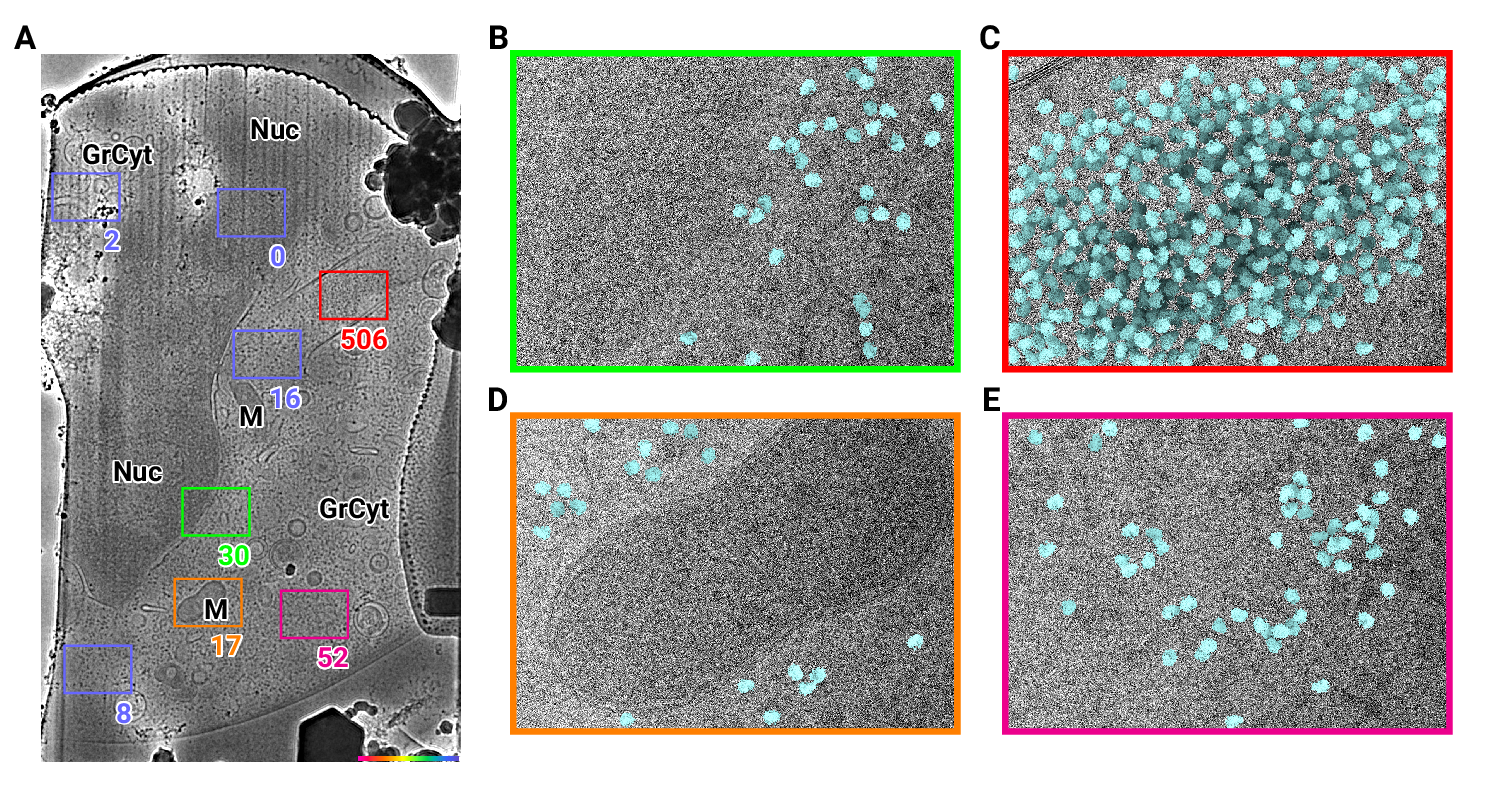
\includegraphics{figures/initmatching.png}
\caption{2D template matching of the large subunit of the ribosome in fib-milled neutrophil-like cells
(A) Overview image of the lamella. Major cellular regions are labeled, as Nucleus (Nuc), Mitochondria (M), and granular cytoplasm (GrCyt). FOVs where high-magnification images for template matching where acquired are indicated as boxes with the number of matches indicated on the bottom right. FOVs displayed in Panels B-E are color-coded.
(B-E) FOVs with projection of ribosome LSU matches shown in green. (B) Perinuclear region, the only matches are in the cytoplasmic half. (C) Cytoplasmic region with high density of ribosomes (D) Mitochondrium, as expected there are only matches in the cytoplasmic region (E) Cytoplasm, with low density of ribosomes.}\label{fig:initmatching}
}
\end{figure}

\begin{fignos:tagged-figure}[S1]

\begin{figure}
\hypertarget{fig:initmatching2}{%
\centering
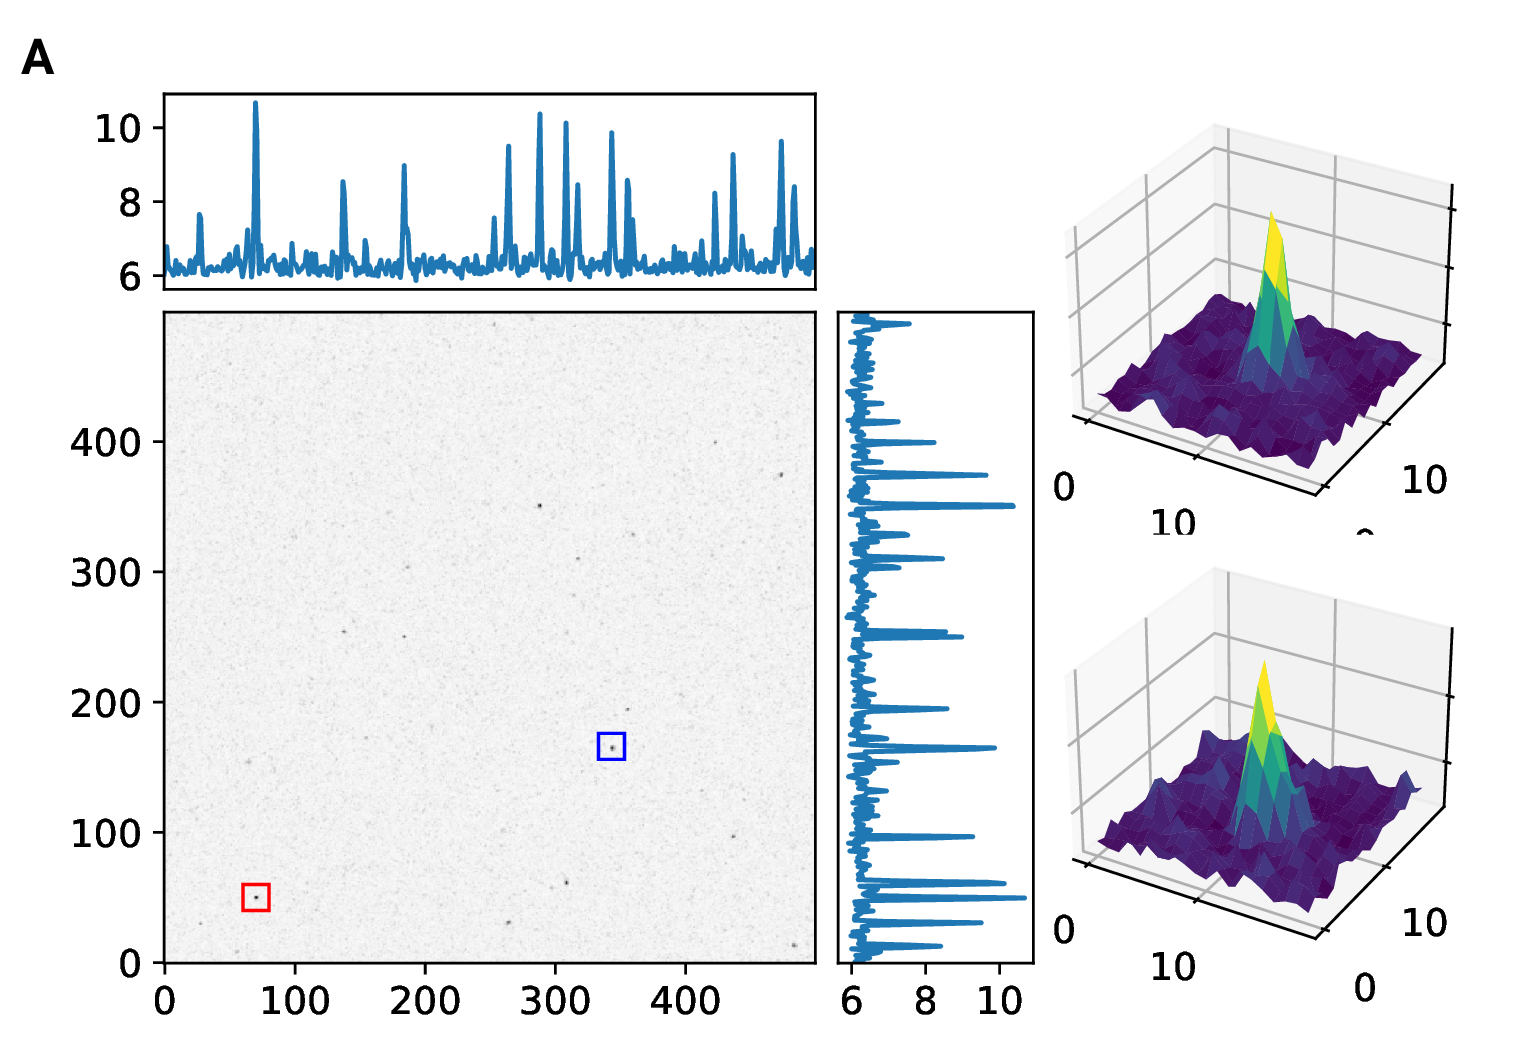
\includegraphics{figures/initmatching2.png}
\caption{2D template matching of the large subunit of the ribosome in fib-milled
neutrophil-like cells (A) Maximum intensity projection cross-correlation map of
micrograph shown in Figure
\ref{fig:initmatching} (B+C) 3D plot of MIP regions indicated by color boxes in Panel A}\label{fig:initmatching2}
}
\end{figure}

\end{fignos:tagged-figure}

\begin{figure}
\hypertarget{fig:approach}{%
\centering
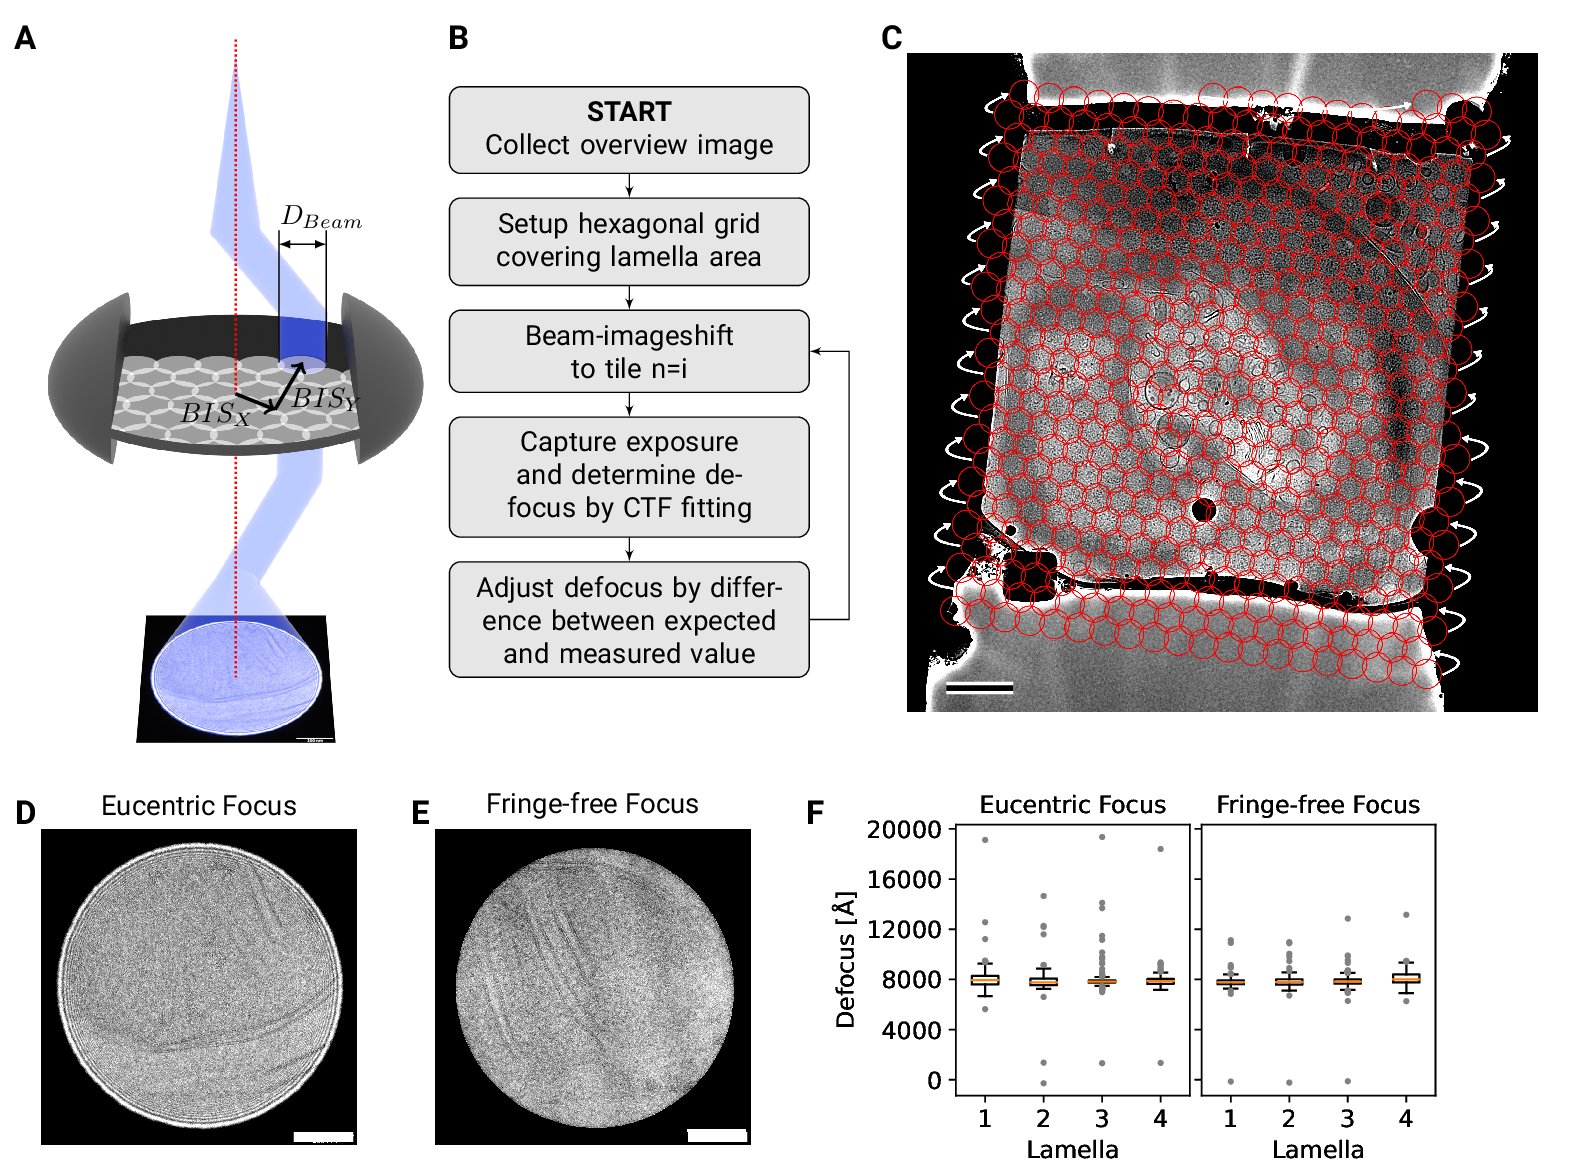
\includegraphics{figures/approach.png}
\caption{DeCo-LACE approach (A) Graphic demonstrating the data-collection strategy for
DeCo-LACE. The electron beam is condensed to a diameter \(D_{Beam}\) that allows captured of
the whole illuminated area on the camera. Beam-image shift along X and Y
(\(BIS_X\),\$\(BIS_Y\)) is used to raster the whole lamella
(B) Diagram of the collection algorithm
(C) Example overview image of a lamella with the designated acquisition
positions and the used beam diameter indicated with red circles
(D+E) Representative micrographs takne with a condensed beam at eucentric focus
(D) or fringe-free focus (E)
(F) Boxplot of defocus measured by ctffind of micrographs taken by the DeCo-Lace
approach on 4 lamella images at eucentric focus and 4 lamella imaged with
fringe-free focus.
(F+G) Lamella overview images of lamella imaged at eucentric focus (F) Overview
image taken at low magnification (40Å pixel size) (G) Overview created by
montaging high magnification images taken with the DeCo-Lace approach (1.5Å
pixelsize)
(H+I) Lamella overview images of lamella imaged at fringe-free focus (H) Overview
image taken at low magnification (40Å pixel size) (I) Overview created by
montaging high magnification images taken with the DeCo-Lace approach (1.5Å
pixelsize)}\label{fig:approach}
}
\end{figure}

\begin{fignos:tagged-figure}[S2]

\begin{figure}
\hypertarget{fig:lamella_images}{%
\centering
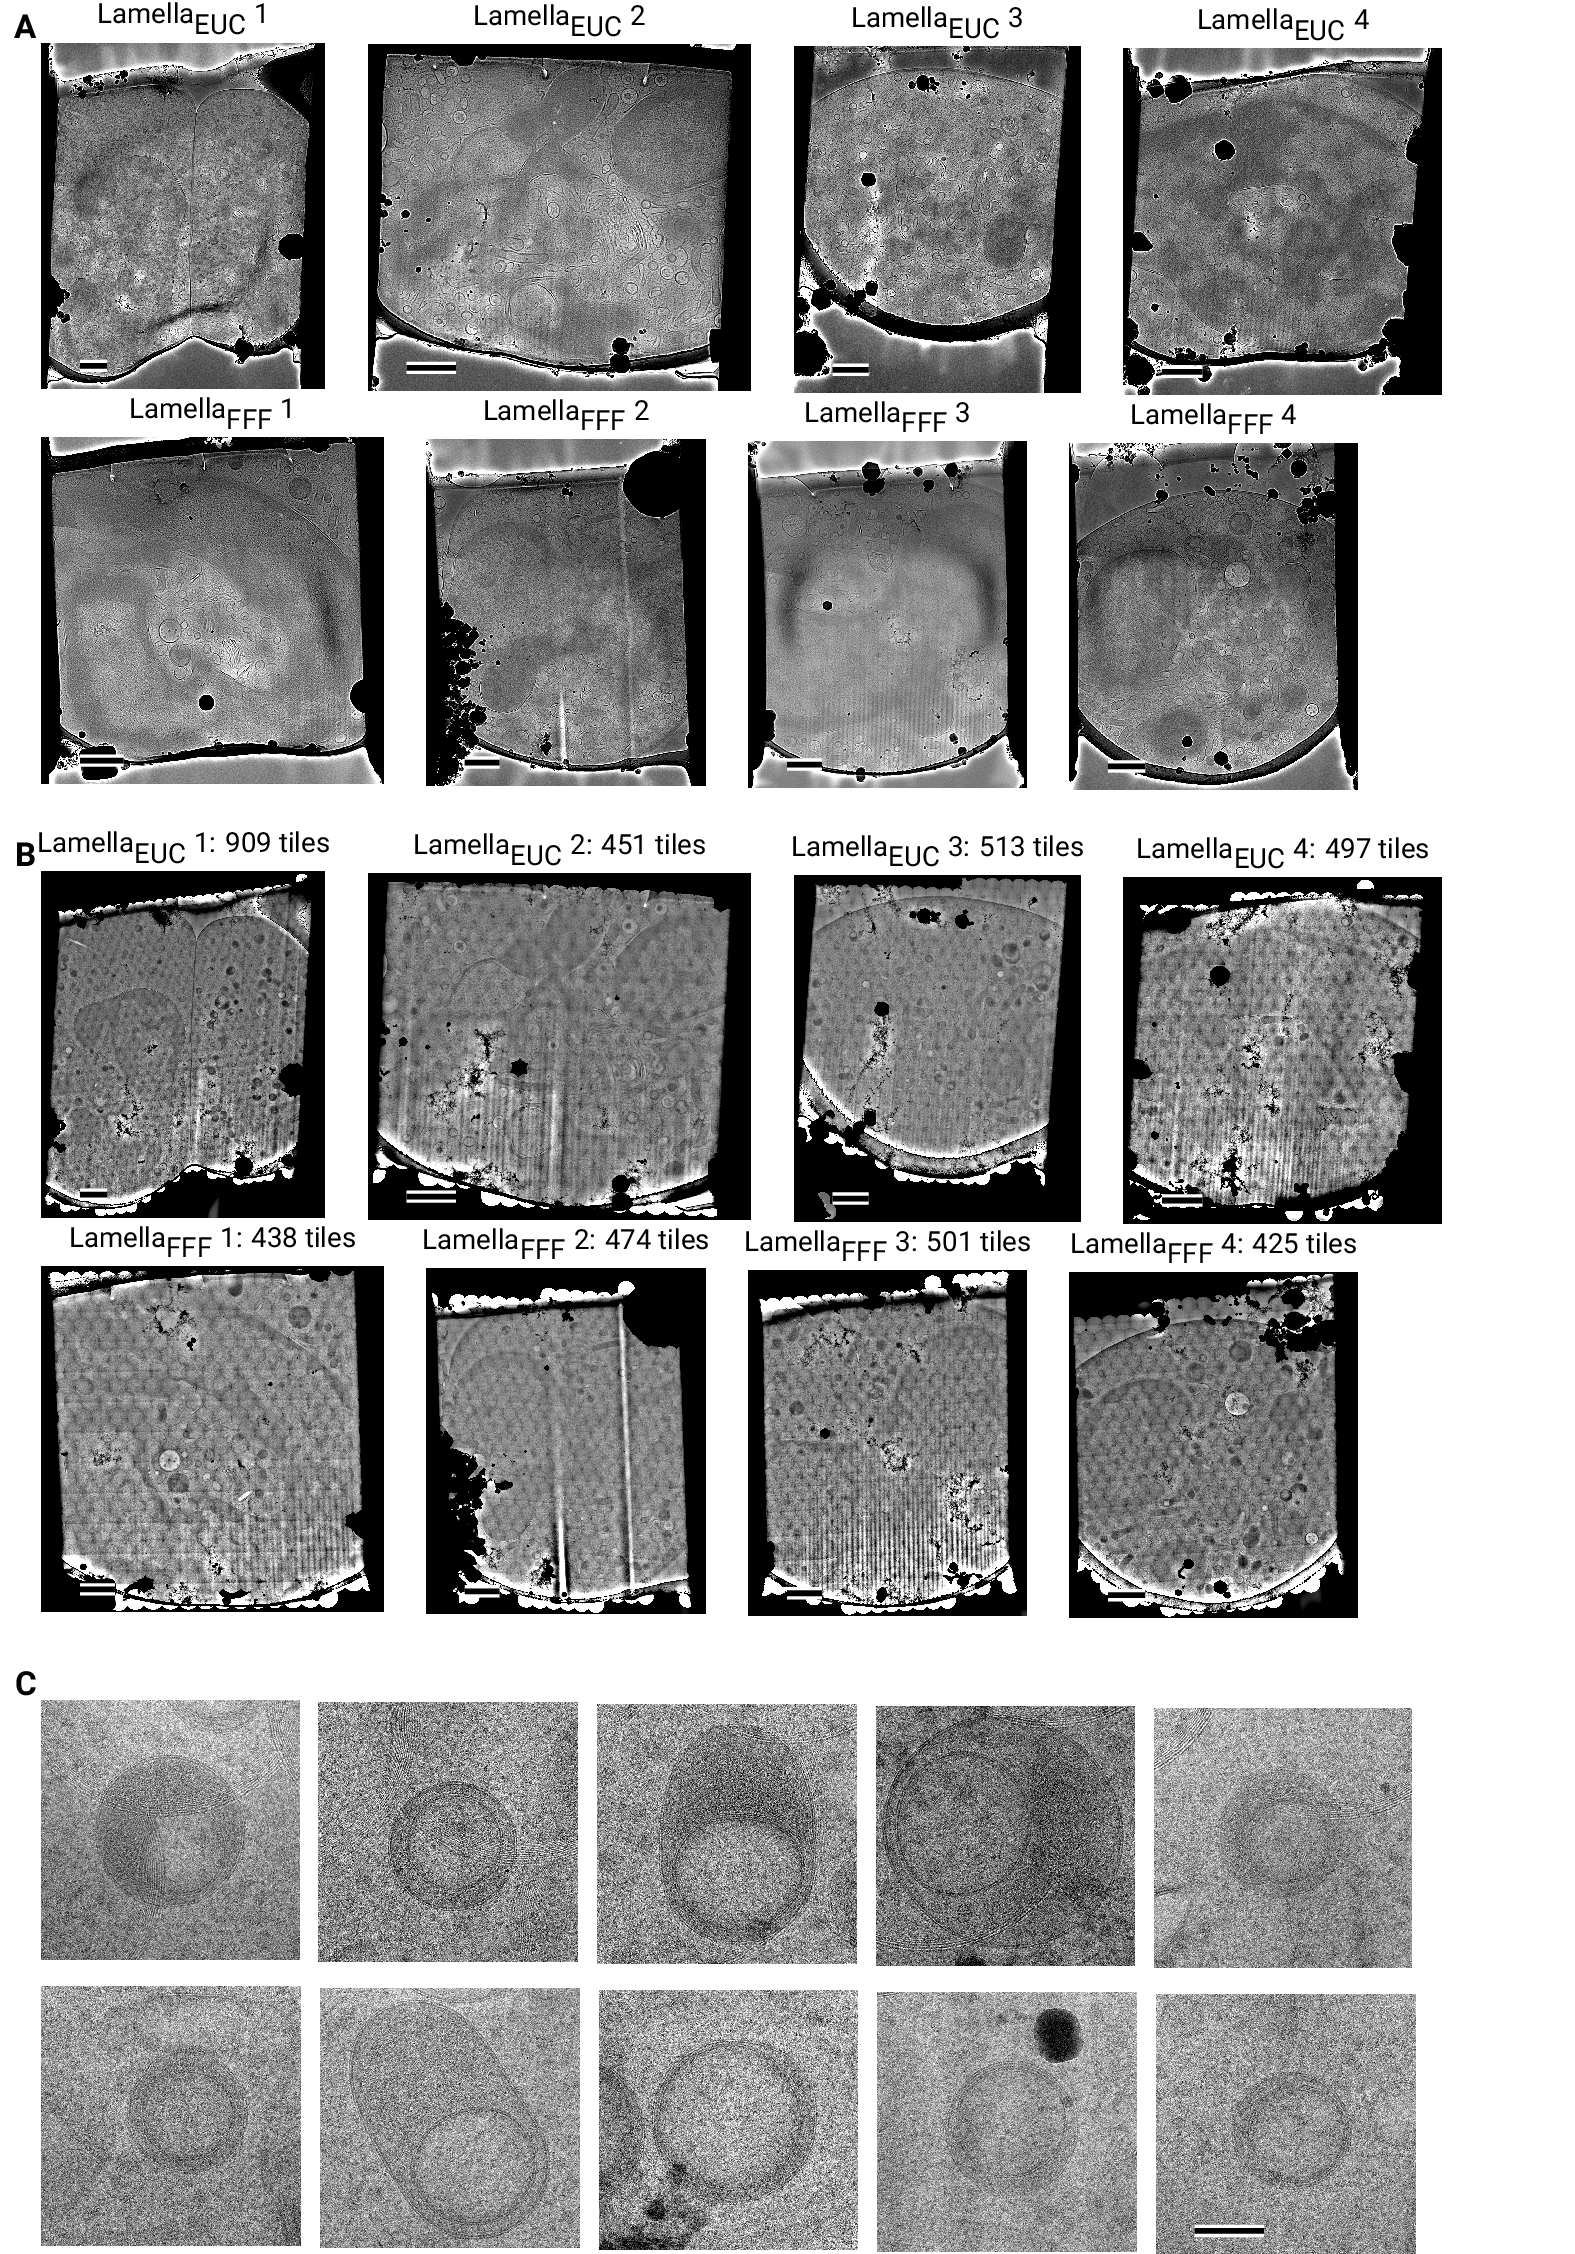
\includegraphics{figures/lamella_images.png}
\caption{Overview images of lamellae imaged using the DeCo-LACE approach taken at low-magnification}\label{fig:lamella_images}
}
\end{figure}

\end{fignos:tagged-figure}

\begin{fignos:tagged-figure}[S3]

\begin{figure}
\hypertarget{fig:lamella_spatial_info}{%
\centering
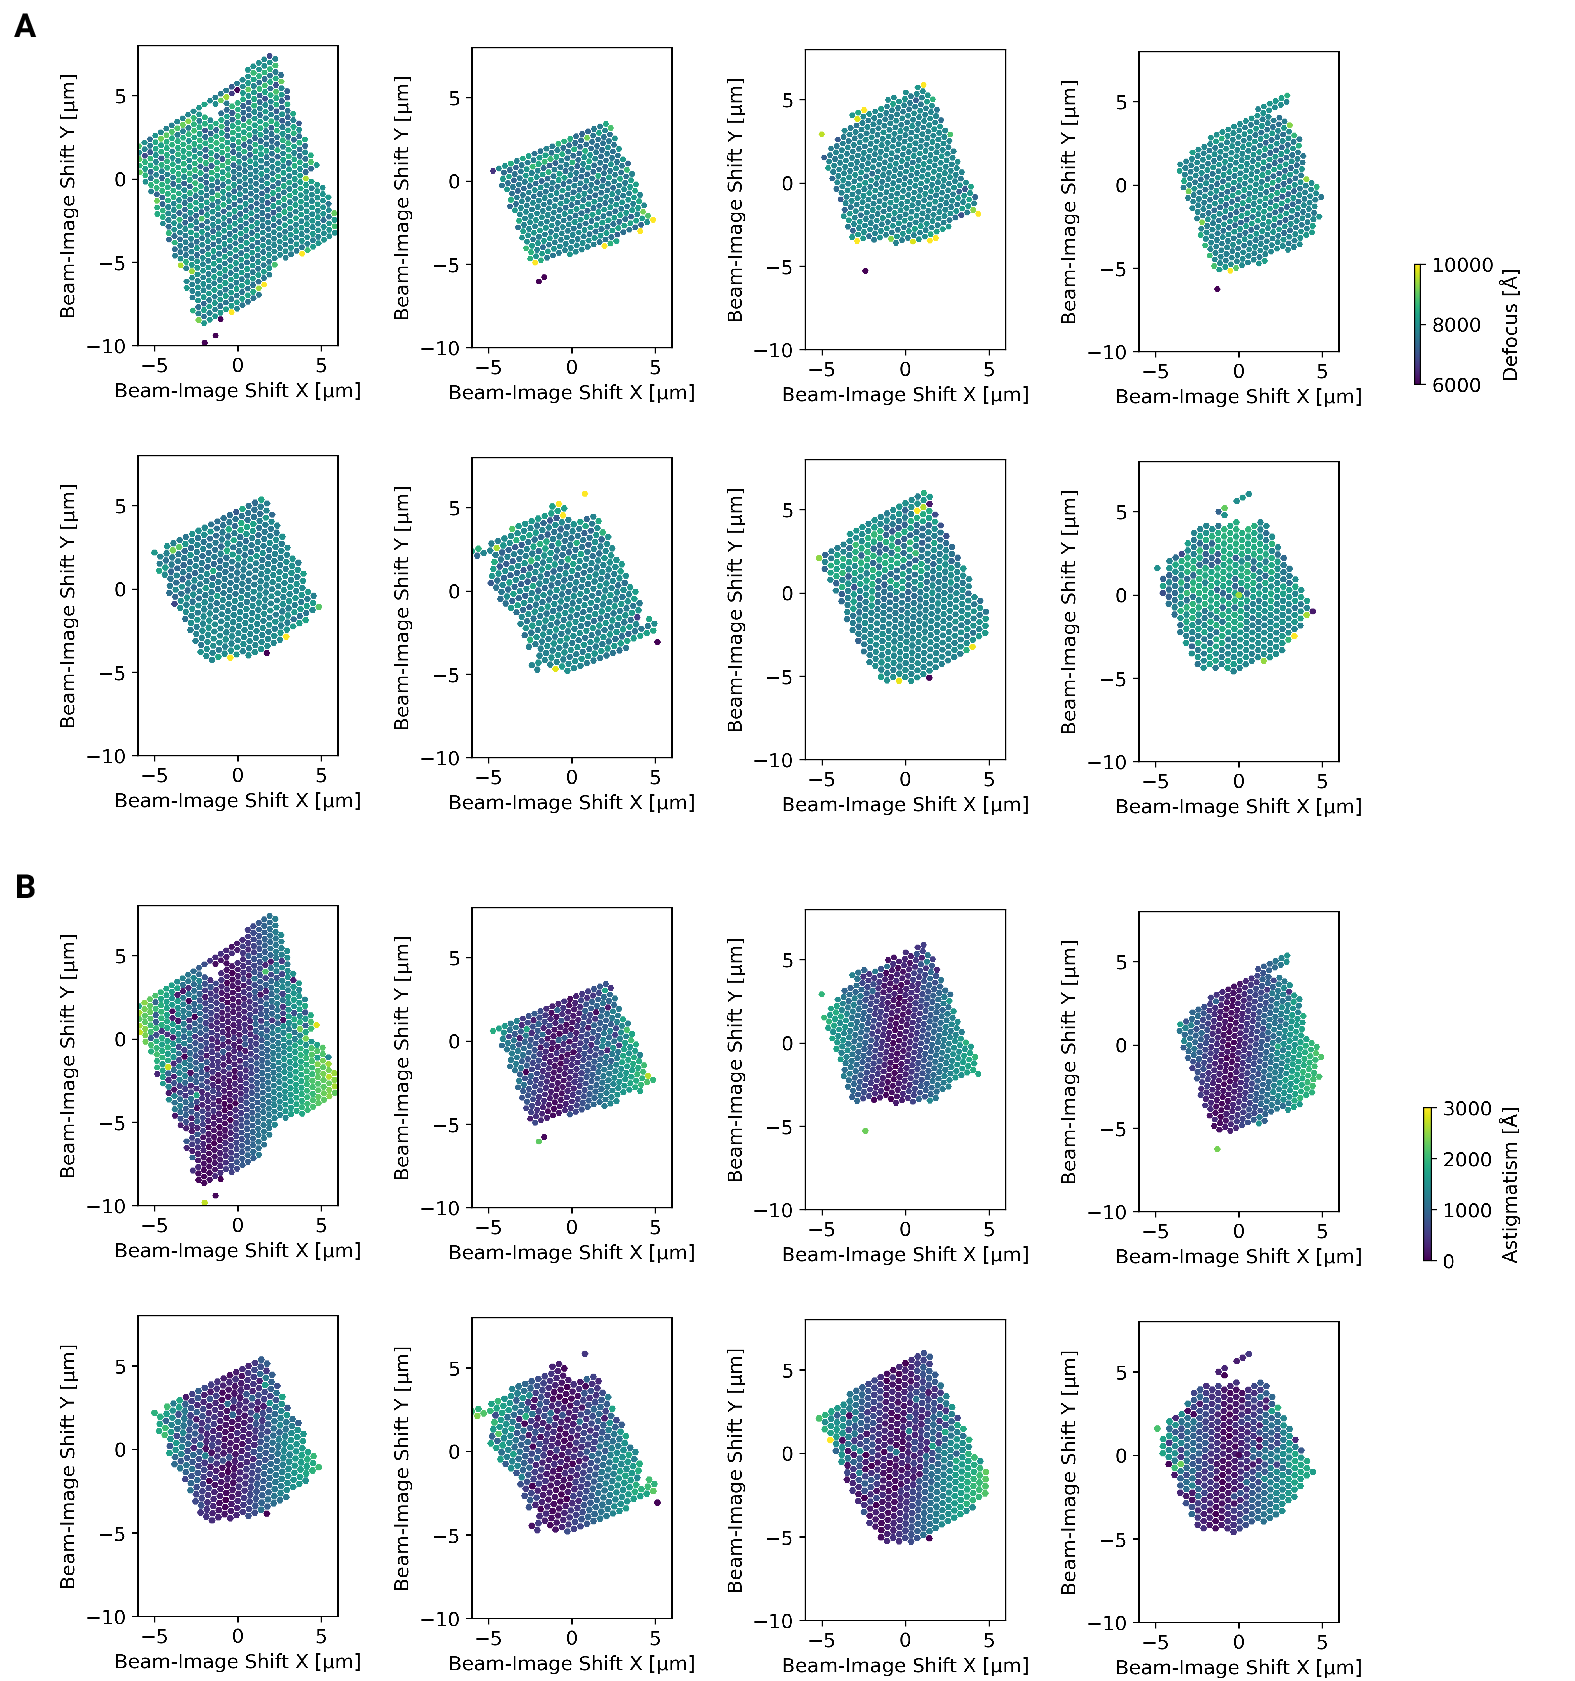
\includegraphics{figures/lamella_spatial_info.png}
\caption{Defocus estimation of individual tiles of DeCo-Lace montages
(A) Defocus values of individual micrographs taken using the DeCo-Lace approach
plotted as a function of the Beam-Image-Shift values.
(B) Defocus astigmatism of individual micrographs taken using the DeCo-Lace approach
plotted as a function of the Beam-Image-Shift values.}\label{fig:lamella_spatial_info}
}
\end{figure}

\end{fignos:tagged-figure}

\begin{fignos:tagged-figure}[S4]

\begin{figure}
\hypertarget{fig:crop_unblur}{%
\centering
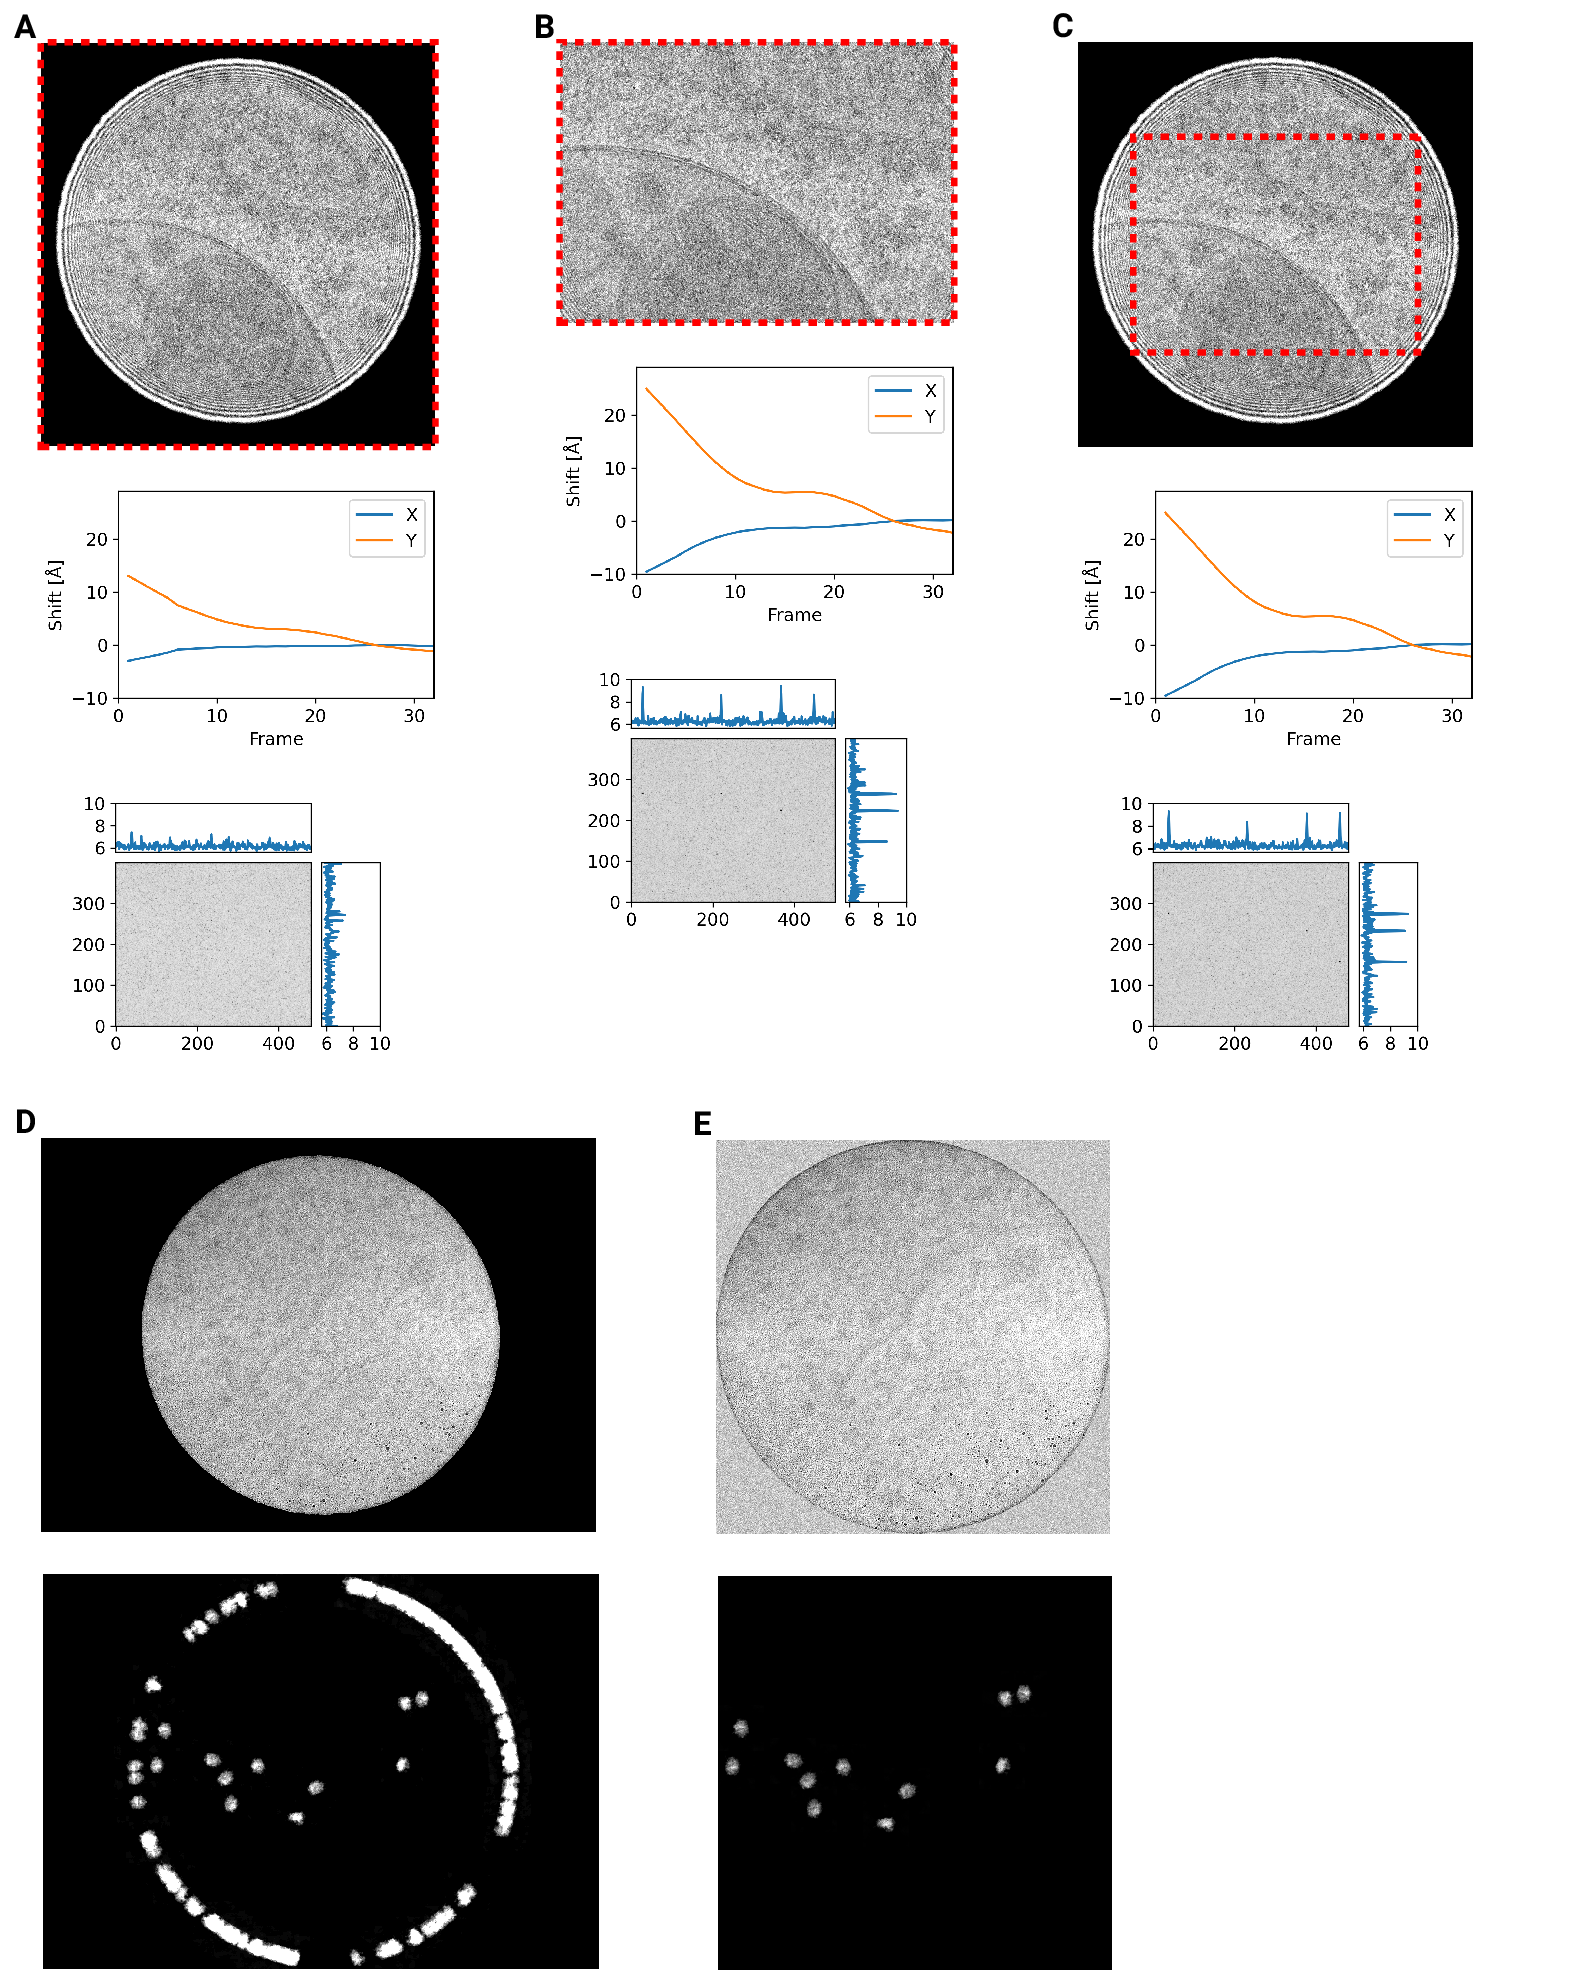
\includegraphics{figures/crop_unblur.png}
\caption{Motion correction of movies with condensed beams.
At the top of each panel is an average of the movie that was motion-corrected
with a red dashed box indicating the region that was used to estimate shifts.
Below is a graph indicating the estimated shifts of the individual frames of the
movie. Below this is the MIP of 2DTM using the large subunit of the mouse ribosome.
(A) Motion correction of the whole movie
(B) Notion correction of a cropped region of the movie that eliminates the beam
edges
(C) Motion correction of the whole movie, using only hte cropped region to
estimate the shifts}\label{fig:crop_unblur}
}
\end{figure}

\end{fignos:tagged-figure}

\begin{fignos:tagged-figure}[S5]

\begin{figure}
\hypertarget{fig:lamella_motion_thickness}{%
\centering
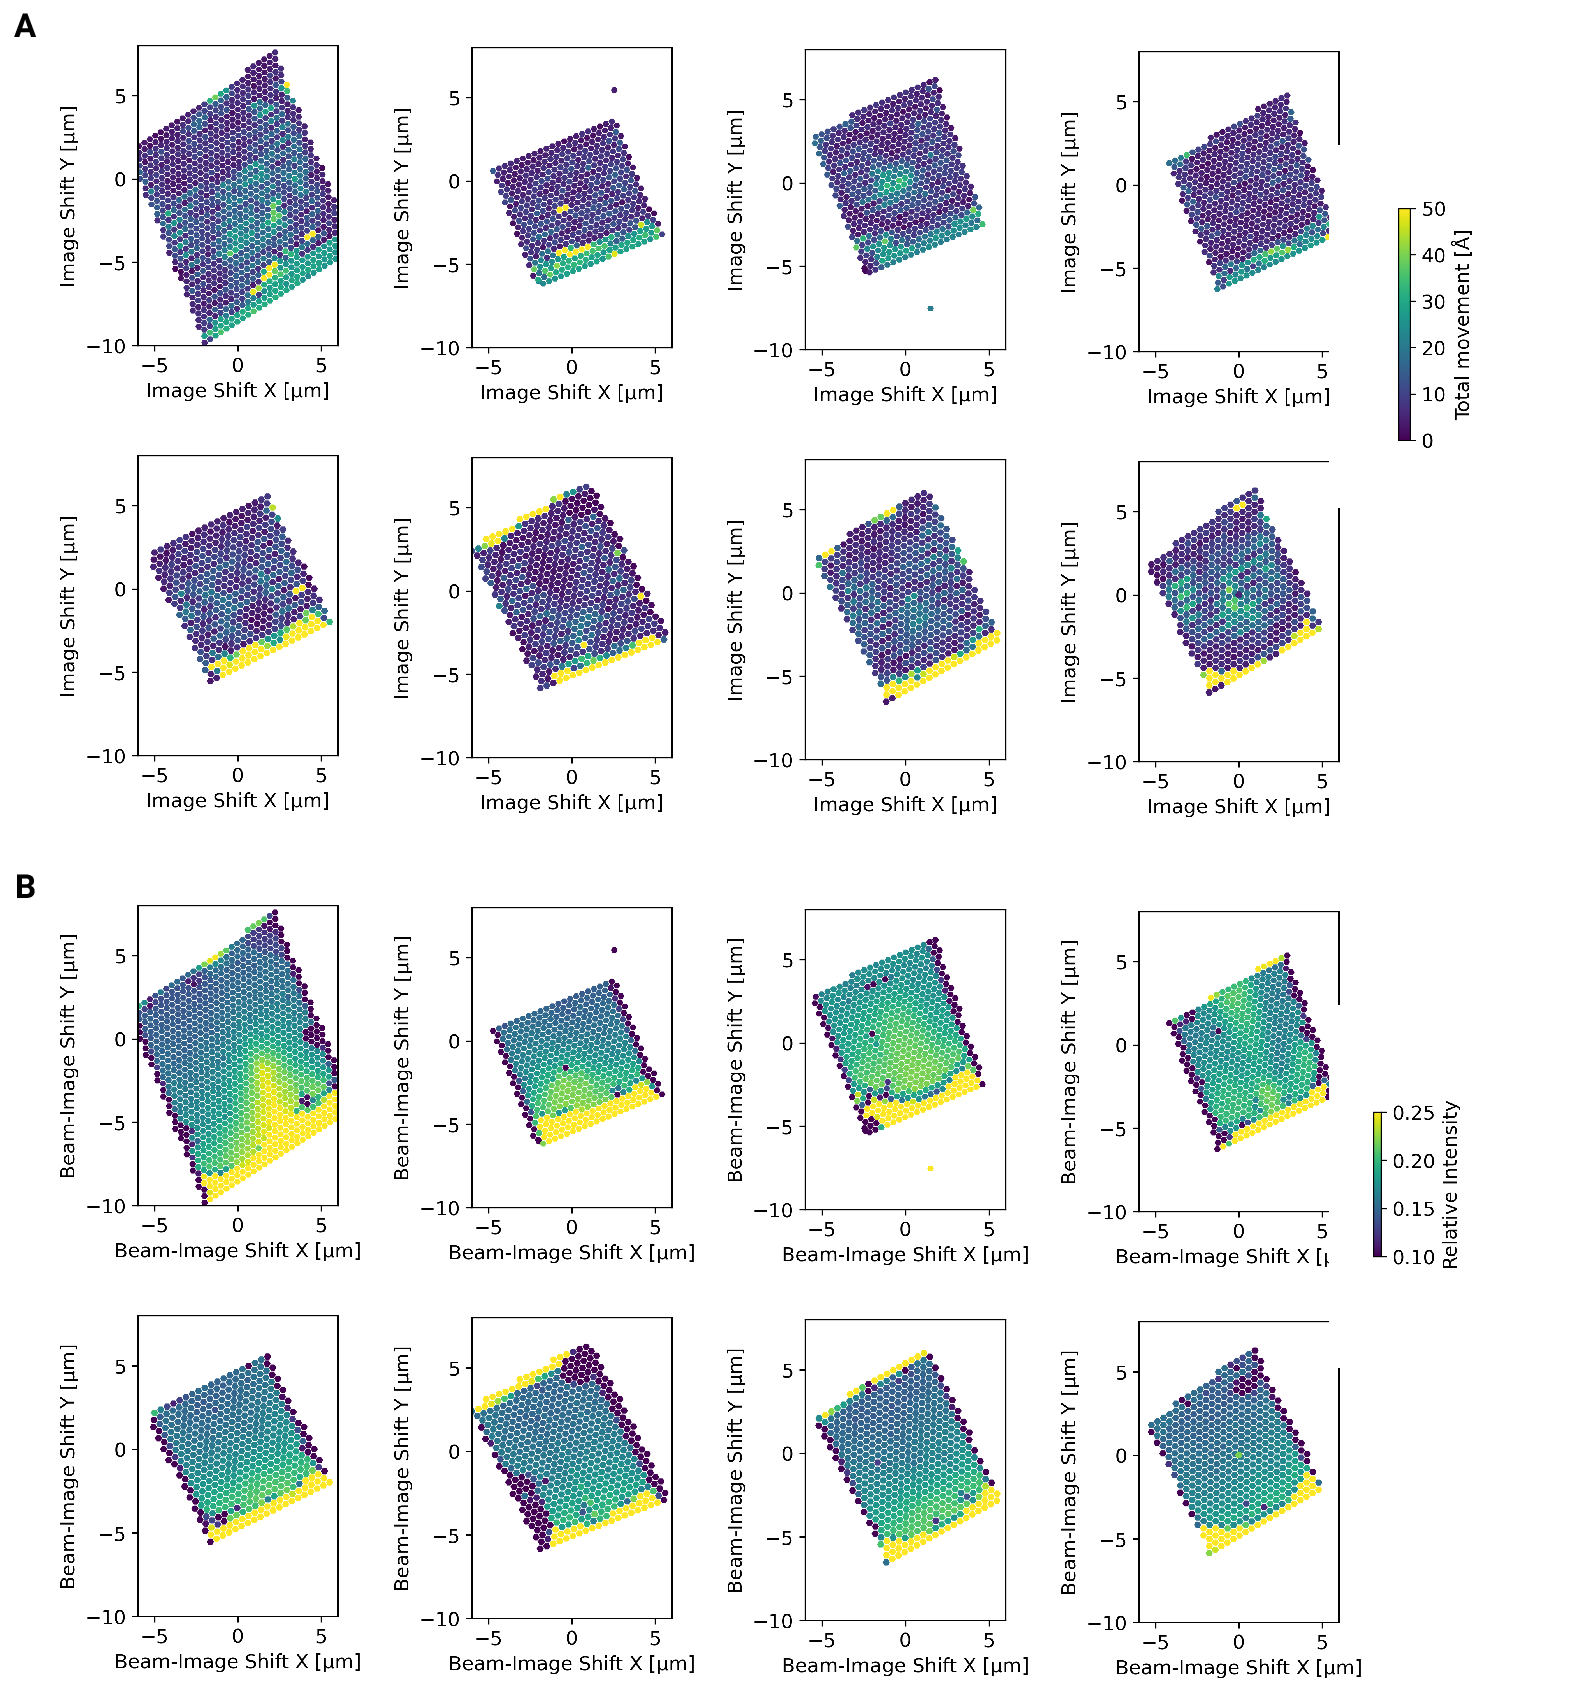
\includegraphics{figures/lamella_motion_thickness.png}
\caption{Motion correction of individual tiles imaged using the DeCo-LACE approach
(A) Total estimated motion of individual micrographs taken using the DeCo-Lace approach
plotted as a function of the Beam-Image-Shift values.
(B) Electron intensity of individual micrographs taken using the DeCo-Lace approach
plotted as a function of the Beam-Image-Shift values.}\label{fig:lamella_motion_thickness}
}
\end{figure}

\end{fignos:tagged-figure}

\begin{figure}
\hypertarget{fig:matching_stat}{%
\centering
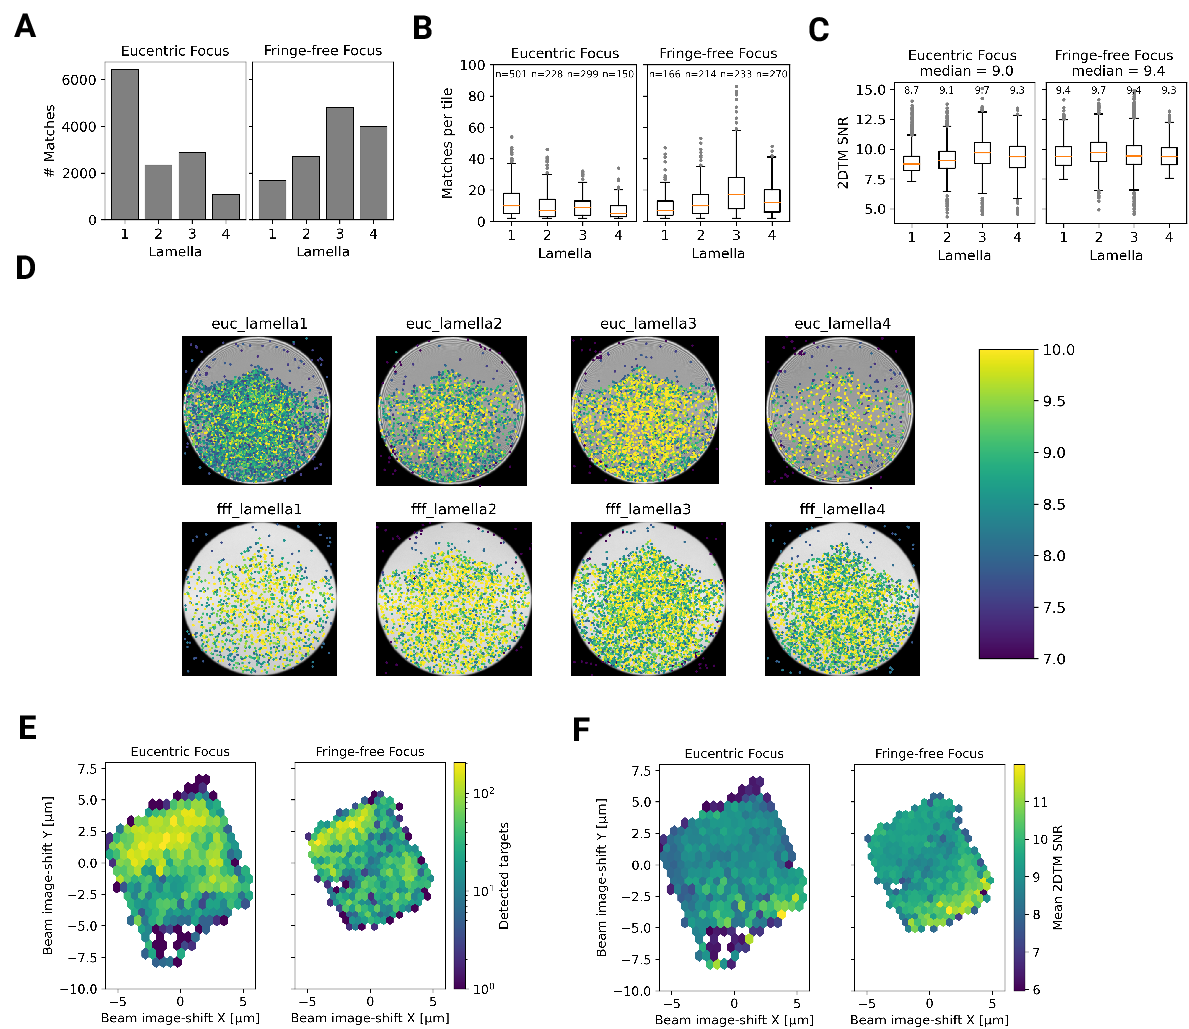
\includegraphics{figures/matching_stat.png}
\caption{Statistics of 2DTM on lamella imaged using DeCo-LACE (A) Number of matches of
each lamella (B) Distribution of matches per tile in each lamella. Only tiles
with two or more matches were included (C) Distribution of SNRs in each lamella
(D) For each lamella an average of all tiles is shown. Overlaid is a scatterplot
of all matches in these tiles according to their in-tile coordinates.
Scatterplot is color according to the SNR. There are no matches in the top
circle-circle intersection due to radiation damage from previous exposures.}\label{fig:matching_stat}
}
\end{figure}

\begin{figure}
\hypertarget{fig:matching_euc}{%
\centering
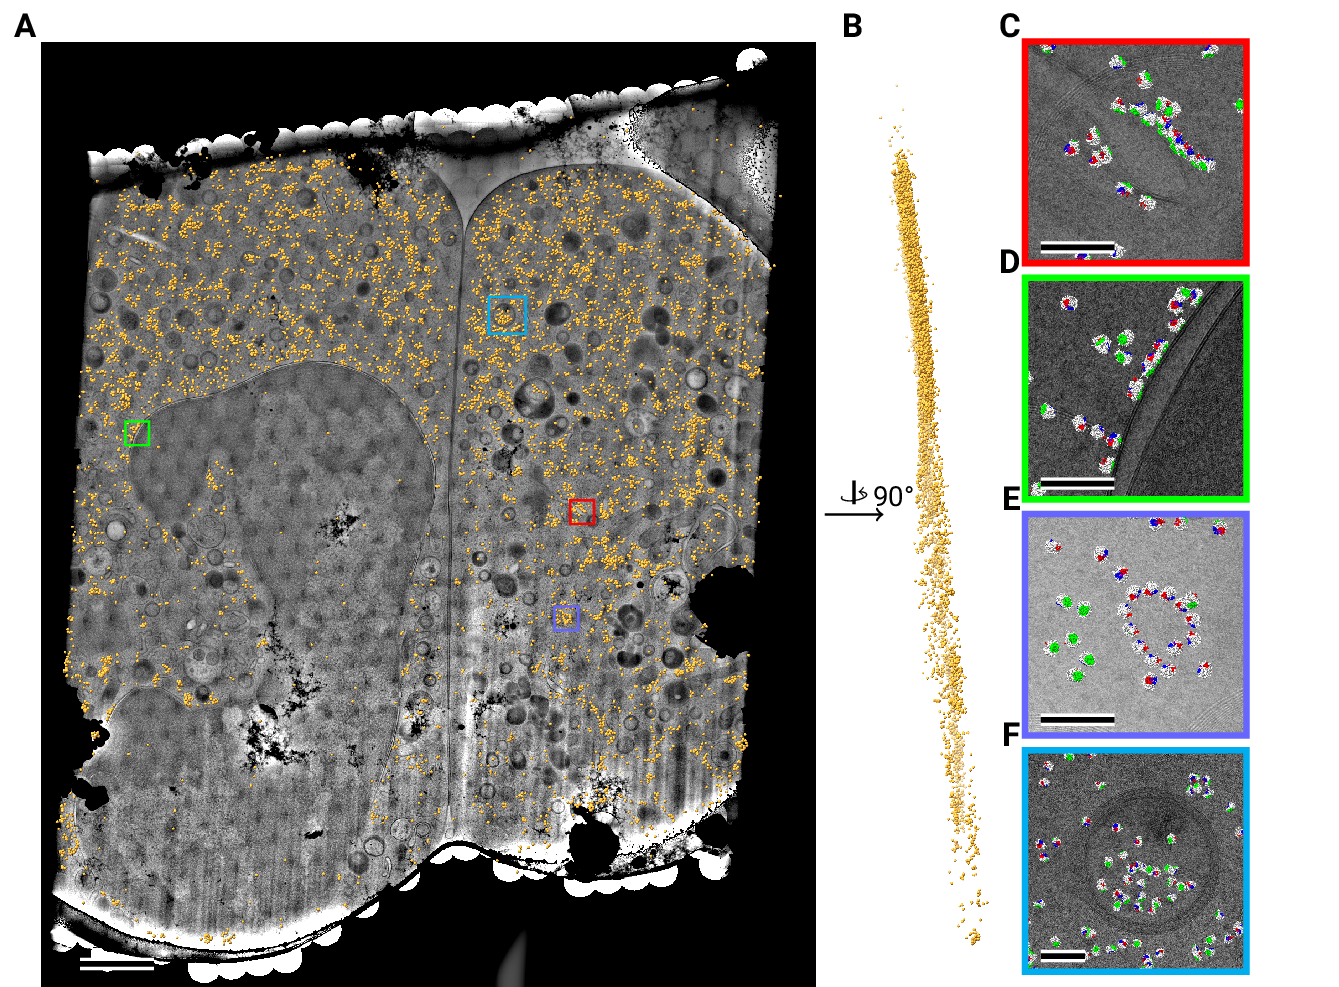
\includegraphics{figures/matching_euc.png}
\caption{Template matching in lamella imaged using the DeCo-Lace approach at eucentric
focus (A) Montage of Lamella\(_\textrm{EUC}\) 1 overlaid with matches according to
their montage coordinates (B) Side view of matches in the lamella, such that the
direction of the electron beam is horizontal. (C-F) Magnified area of panel A
showing rough ER with associated ribosomes(C), outer nuclear membrane with
associated ribosomes (D), ribsomes arranged in a circular fashion(E), ribosomes
enclosed in a less electron dense inclusion in a granule(F).}\label{fig:matching_euc}
}
\end{figure}

\begin{figure}
\hypertarget{fig:matching_fff}{%
\centering
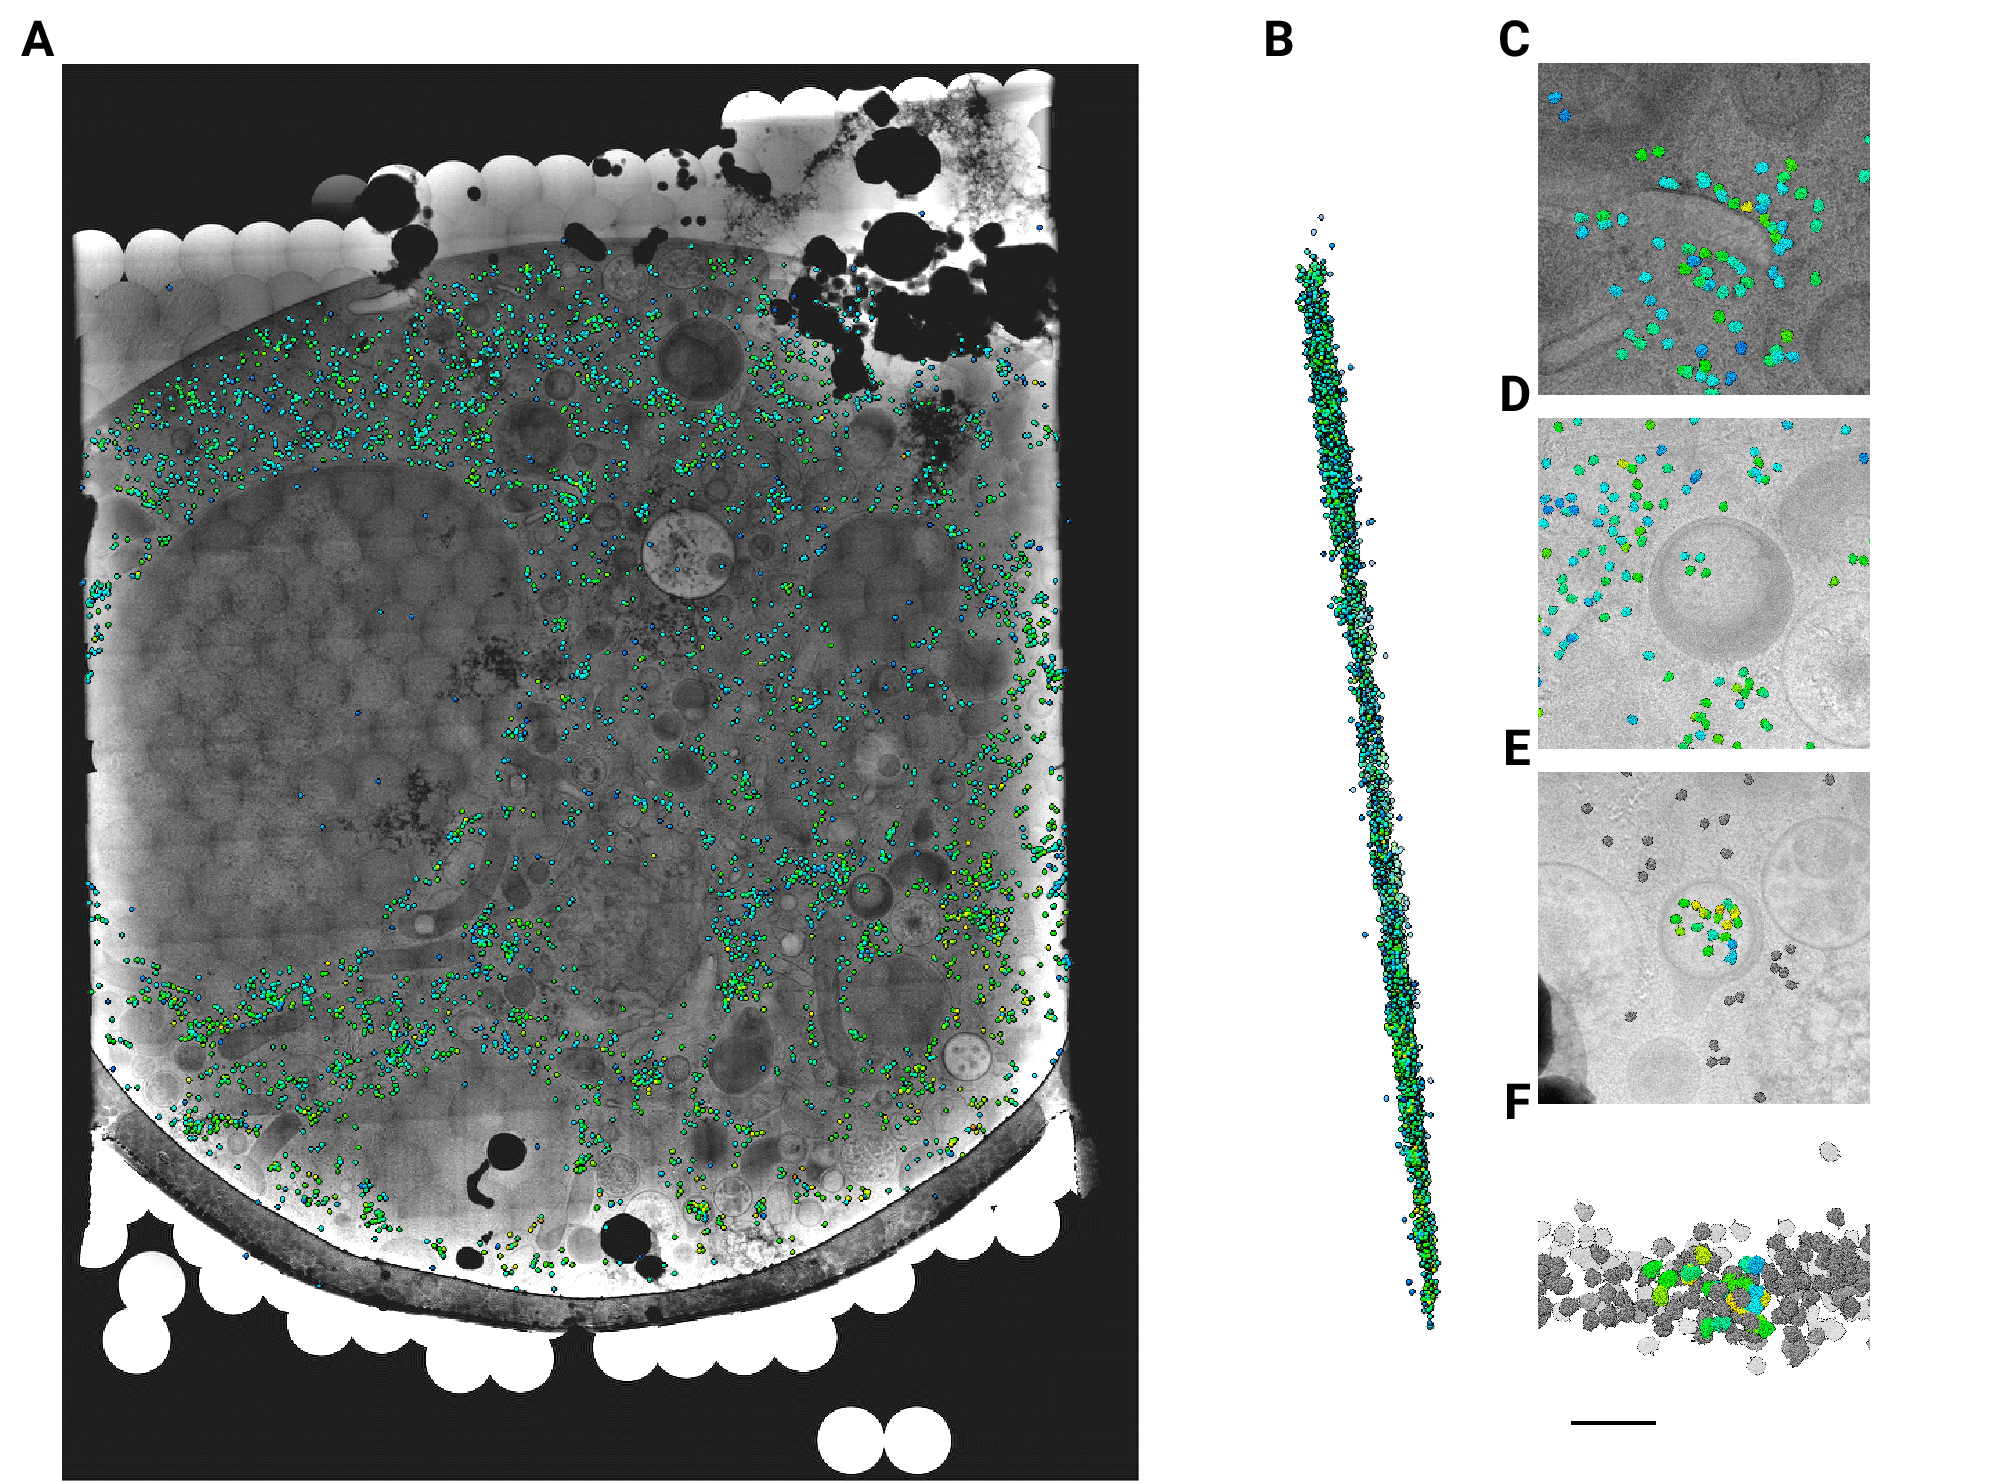
\includegraphics{figures/matching_fff.png}
\caption{Template matching in lamella imaged using the DeCo-Lace approach at fringe-free
focus (A) Montage of Lamella\(_\textrm{FFF}\) 4 overlaid with matches according to
their montage coordinates (B) Side view of matches in the lamella, such that the
direction of the electron beam is horizontal. (C-E) Magnified area of panel A
showing rough ER with associated ribosomes(C) and ribosomes
enclosed in a less electron dense inclusion in a granule(D,E). (F) Side view of
panel E with ribosomes situated inside the granule colored accoding
to SNR and other ribosomes colored in grey.}\label{fig:matching_fff}
}
\end{figure}

\begin{figure}
\hypertarget{fig:deco_lace_workflow}{%
\centering
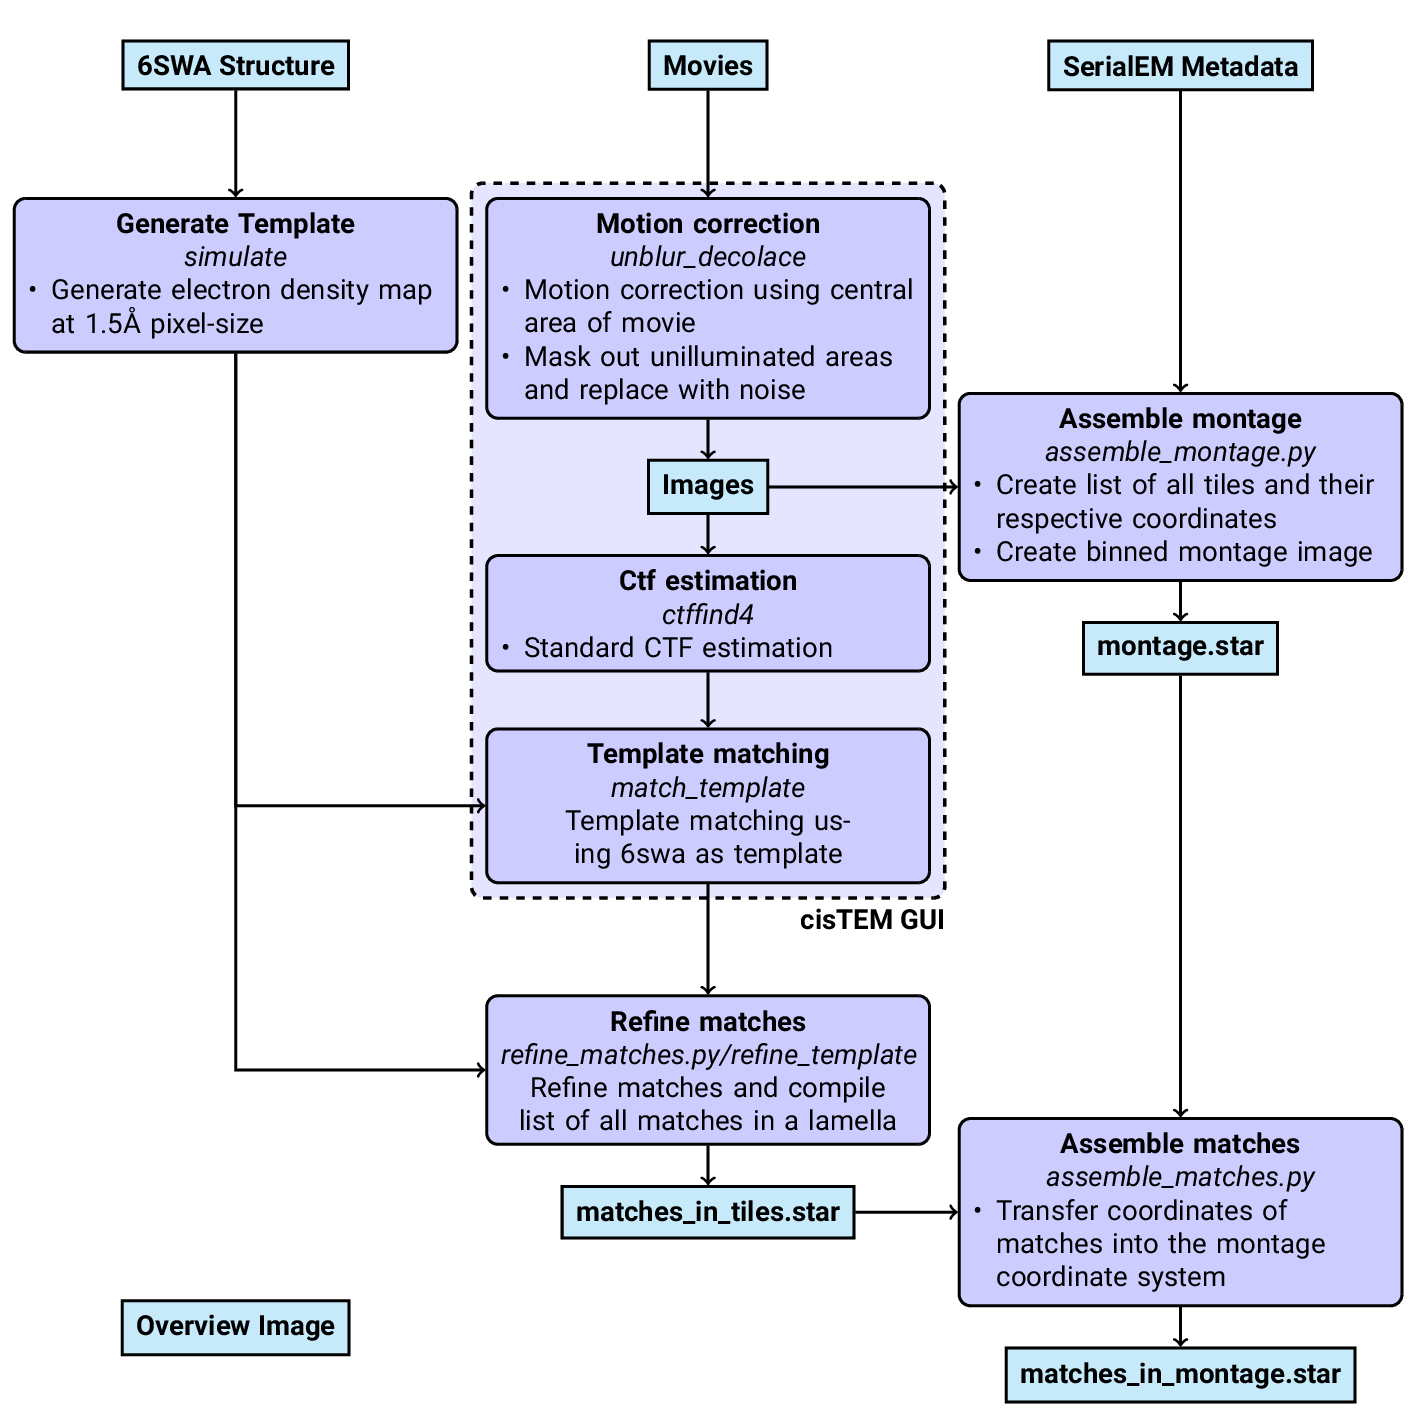
\includegraphics{figures/deco_lace_workflow.png}
\caption{Workflow of DeCo-Lace processing}\label{fig:deco_lace_workflow}
}
\end{figure}

\hypertarget{references}{%
\subsection{References}\label{references}}

\hypertarget{refs}{}
\begin{CSLReferences}{0}{0}
\leavevmode\vadjust pre{\hypertarget{ref-tSXIKPl7}{}}%
\CSLLeftMargin{1. }%
\CSLRightInline{\textbf{Label-free, normalized quantification of complex mass spectrometry data for proteomic analysis}
\CSLBlock{Noelle M Griffin, Jingyi Yu, Fred Long, Phil Oh, Sabrina Shore, Yan Li, Jim A Koziol, Jan E Schnitzer} \emph{Nature Biotechnology} (2010-01) \url{https://doi.org/fshgnc}
\CSLBlock{DOI: \href{https://doi.org/10.1038/nbt.1592}{10.1038/nbt.1592} · PMID: \href{https://www.ncbi.nlm.nih.gov/pubmed/20010810}{20010810} · PMCID: \href{https://www.ncbi.nlm.nih.gov/pmc/articles/PMC2805705}{PMC2805705}}}

\leavevmode\vadjust pre{\hypertarget{ref-VBmW7Aot}{}}%
\CSLLeftMargin{2. }%
\CSLRightInline{\textbf{Fluorescence microscopy}
\CSLBlock{Jeff W Lichtman, José-Angel Conchello} \emph{Nature Methods} (2005-11-18) \url{https://doi.org/bbpg4n}
\CSLBlock{DOI: \href{https://doi.org/10.1038/nmeth817}{10.1038/nmeth817} · PMID: \href{https://www.ncbi.nlm.nih.gov/pubmed/16299476}{16299476}}}

\leavevmode\vadjust pre{\hypertarget{ref-tGQ6TSUo}{}}%
\CSLLeftMargin{3. }%
\CSLRightInline{\textbf{A visual approach to proteomics}
\CSLBlock{Stephan Nickell, Christine Kofler, Andrew P Leis, Wolfgang Baumeister} \emph{Nature Reviews Molecular Cell Biology} (2006-02-15) \url{https://doi.org/d6d5mq}
\CSLBlock{DOI: \href{https://doi.org/10.1038/nrm1861}{10.1038/nrm1861} · PMID: \href{https://www.ncbi.nlm.nih.gov/pubmed/16482091}{16482091}}}

\leavevmode\vadjust pre{\hypertarget{ref-g8QavfwP}{}}%
\CSLLeftMargin{4. }%
\CSLRightInline{\textbf{Electron microscopy of frozen hydrated sections of vitreous ice and vitrified biological samples}
\CSLBlock{AW McDowall, J-J Chang, R Freeman, J Lepault, CA Walter, J Dubochet} \emph{Journal of Microscopy} (1983-07) \url{https://doi.org/bdnzmv}
\CSLBlock{DOI: \href{https://doi.org/10.1111/j.1365-2818.1983.tb04225.x}{10.1111/j.1365-2818.1983.tb04225.x} · PMID: \href{https://www.ncbi.nlm.nih.gov/pubmed/6350598}{6350598}}}

\leavevmode\vadjust pre{\hypertarget{ref-16IhS1Nc4}{}}%
\CSLLeftMargin{5. }%
\CSLRightInline{\textbf{Opening windows into the cell: focused-ion-beam milling for cryo-electron tomography}
\CSLBlock{Elizabeth Villa, Miroslava Schaffer, Jürgen M Plitzko, Wolfgang Baumeister} \emph{Current Opinion in Structural Biology} (2013-10) \url{https://doi.org/f537jp}
\CSLBlock{DOI: \href{https://doi.org/10.1016/j.sbi.2013.08.006}{10.1016/j.sbi.2013.08.006} · PMID: \href{https://www.ncbi.nlm.nih.gov/pubmed/24090931}{24090931}}}

\leavevmode\vadjust pre{\hypertarget{ref-Rksh2dxu}{}}%
\CSLLeftMargin{6. }%
\CSLRightInline{\textbf{Electron tomography of cells}
\CSLBlock{Lu Gan, Grant J Jensen} \emph{Quarterly Reviews of Biophysics} (2011-11-15) \url{https://doi.org/czj9hr}
\CSLBlock{DOI: \href{https://doi.org/10.1017/s0033583511000102}{10.1017/s0033583511000102} · PMID: \href{https://www.ncbi.nlm.nih.gov/pubmed/22082691}{22082691}}}

\leavevmode\vadjust pre{\hypertarget{ref-Ynb3IP6I}{}}%
\CSLLeftMargin{7. }%
\CSLRightInline{\textbf{Single-protein detection in crowded molecular environments in cryo-EM images}
\CSLBlock{JPeter Rickgauer, Nikolaus Grigorieff, Winfried Denk} \emph{eLife} (2017-05-03) \url{https://doi.org/gnq4q4}
\CSLBlock{DOI: \href{https://doi.org/10.7554/elife.25648}{10.7554/elife.25648} · PMID: \href{https://www.ncbi.nlm.nih.gov/pubmed/28467302}{28467302} · PMCID: \href{https://www.ncbi.nlm.nih.gov/pmc/articles/PMC5453696}{PMC5453696}}}

\leavevmode\vadjust pre{\hypertarget{ref-18KGpXYPE}{}}%
\CSLLeftMargin{8. }%
\CSLRightInline{\textbf{Label-free single-instance protein detection in vitrified cells}
\CSLBlock{JPeter Rickgauer, Heejun Choi, Jennifer Lippincott-Schwartz, Winfried Denk} \emph{Cold Spring Harbor Laboratory} (2020-04-24) \url{https://doi.org/gpbjfd}
\CSLBlock{DOI: \href{https://doi.org/10.1101/2020.04.22.053868}{10.1101/2020.04.22.053868}}}

\leavevmode\vadjust pre{\hypertarget{ref-10bXZuF3G}{}}%
\CSLLeftMargin{9. }%
\CSLRightInline{\textbf{Locating macromolecular assemblies in cells by 2D template matching with cisTEM}
\CSLBlock{Bronwyn A Lucas, Benjamin A Himes, Liang Xue, Timothy Grant, Julia Mahamid, Nikolaus Grigorieff} \emph{eLife} (2021-06-11) \url{https://doi.org/gkkc49}
\CSLBlock{DOI: \href{https://doi.org/10.7554/elife.68946}{10.7554/elife.68946} · PMID: \href{https://www.ncbi.nlm.nih.gov/pubmed/34114559}{34114559} · PMCID: \href{https://www.ncbi.nlm.nih.gov/pmc/articles/PMC8219381}{PMC8219381}}}

\leavevmode\vadjust pre{\hypertarget{ref-gRoY21jY}{}}%
\CSLLeftMargin{10. }%
\CSLRightInline{\textbf{Hallmarks of ribosomopathies}
\CSLBlock{Kim R Kampen, Sergey O Sulima, Stijn Vereecke, Kim De~Keersmaecker} \emph{Nucleic Acids Research} (2019-07-27) \url{https://doi.org/gpbjfm}
\CSLBlock{DOI: \href{https://doi.org/10.1093/nar/gkz637}{10.1093/nar/gkz637} · PMID: \href{https://www.ncbi.nlm.nih.gov/pubmed/31350888}{31350888} · PMCID: \href{https://www.ncbi.nlm.nih.gov/pmc/articles/PMC7026650}{PMC7026650}}}

\leavevmode\vadjust pre{\hypertarget{ref-KAJ7221k}{}}%
\CSLLeftMargin{11. }%
\CSLRightInline{\textbf{Diagnostic and prognostic implications of ribosomal protein transcript expression patterns in human cancers}
\CSLBlock{James M Dolezal, Arie P Dash, Edward V Prochownik} \emph{BMC Cancer} (2018-03-12) \url{https://doi.org/gc87j9}
\CSLBlock{DOI: \href{https://doi.org/10.1186/s12885-018-4178-z}{10.1186/s12885-018-4178-z} · PMID: \href{https://www.ncbi.nlm.nih.gov/pubmed/29530001}{29530001} · PMCID: \href{https://www.ncbi.nlm.nih.gov/pmc/articles/PMC5848553}{PMC5848553}}}

\leavevmode\vadjust pre{\hypertarget{ref-1B9Vt9eYu}{}}%
\CSLLeftMargin{12. }%
\CSLRightInline{\textbf{Inhibition of Dihydroorotate Dehydrogenase Overcomes Differentiation Blockade in Acute Myeloid Leukemia}
\CSLBlock{David B Sykes, Youmna S Kfoury, François E Mercier, Mathias J Wawer, Jason M Law, Mark K Haynes, Timothy A Lewis, Amir Schajnovitz, Esha Jain, Dongjun Lee, \ldots{} David T Scadden} \emph{Cell} (2016-09) \url{https://doi.org/f3r5jr}
\CSLBlock{DOI: \href{https://doi.org/10.1016/j.cell.2016.08.057}{10.1016/j.cell.2016.08.057} · PMID: \href{https://www.ncbi.nlm.nih.gov/pubmed/27641501}{27641501} · PMCID: \href{https://www.ncbi.nlm.nih.gov/pmc/articles/PMC7360335}{PMC7360335}}}

\end{CSLReferences}

\end{document}
